\documentclass{beamerthemeMono}

% specify some optional logos
\graphicspath{{figures/}}
%\pgfdeclareimage[height=1.45cm]{mainlogo}{figures/logo}
\pgfdeclareimage[height=1.4cm]{mainlogo}{figures/logo.pdf}
% placed in the lower left/right corner if the \pgfuseimage{minilogo}
% command is uncommented in the \institute command below.
\pgfdeclareimage[height=1cm]{minilogo}{figures/logo.pdf}
\logo{\pgfuseimage{minilogo}}

\AtBeginSection[] {
  \begin{frame}
    \frametitle{目录} 
    {\tableofcontents[%
      currentsection, % causes all sections but the current to be shown in a semi-transparent way.
%     currentsubsection, % causes all subsections but the current subsection in the current section to ...
      hideallsubsections, % causes all subsections to be hidden.
%     hideothersubsections, % causes the subsections of sections other than the current one to be hidden.
%      part=2 % part number causes the table of contents of part part number to be shown
%     pausesections, % causes a \pause command to be issued before each section. This is useful if you
%     pausesubsections, %  causes a \pause command to be issued before each subsection.
      %sections={<1-3|handout:0>} %{ overlay specification },
      ]}
   \end{frame}}

\makeatletter
\AtBeginPart{%
  \beamer@tocsectionnumber=0\relax
  \setcounter{section}{0}
  \frame[plain]{\partpage}%
}
\makeatother

% \AtBeginPart{
%      \begin{frame}[plain]
%          \partpage
%      \end{frame}}

% \AtBeginSubsection[]                            % 在每个子段落之前
% {
%   \frame{                                         % handout:0 表示只在手稿中出现
%     \frametitle{目录} \small
%     \tableofcontents[
%       currentsection,
%       currentsubsection,
%       subsectionstyle=show/shaded/hide]
%   }
% }
%%%%%%%%%%%%%%%%%%%%%%%%%%%%%%%%%%%%%%%%%%%%%%%%%%%%%%%%%%%%
%%%%%%%%%%%%%%%%%%%%%%%%%%%%%%%%%%%%%%%%%%%%%%%%%%%%%%%%%%%%
          % 文档开始
%%%%%%%%%%%%%%%%%%%%%%%%%%%%%%%%%%%%%%%%%%%%%%%%%%%%%%%%%%%%
%%%%%%%%%%%%%%%%%%%%%%%%%%%%%%%%%%%%%%%%%%%%%%%%%%%%%%%%%%%%

 % the titlepage the plain option removes the sidebar and header from
 % the title page
\title[交通规划行业中的数据应用现状及思考]% optional, use only with long paper titles
{\heiti \xiaoerhao 交通规划行业中的数据应用现状及思考}
\date{\xiaosihao 2019年2月}

\author[邹海翔] % optional, use only with lots of authors
{\xiaosihao 邹海翔}

\institute[综合交通所] % optional - is placed in the bottom of the sidebar on every slide
{%
   \xiaosihao 综合交通所
   % there must be an empty line above this line - otherwise some
   % unwanted space is added
   % between the university and the country (I do not know why)
}

\titlegraphic{\pgfuseimage{mainlogo}} %insert a company or department logo

\begin{document}

\RemoveAlgoNumber

\begin{frame}[plain]
  \titlepage
\end{frame}
%%%%%%%%%%%%%%%%


\begin{frame}{大纲}{}
   {\tableofcontents[hideallsubsections]}
\end{frame}

%
%%% Local Variables:
%%% mode: latex
%%% TeX-master: t
%%% End:
%%%%%%%%%%%%%%%%%%%%%%%%%%%%%%%%%%%%%%%%%%%%%%%%%%%%%%%%%%%%

%%%%%%%%%%%%%%%%%%%%%%%%%%%%%%%%%%%%%%%%%%%%%%%%%%%%%%%%%%%%
\section{大数据时代下的交通规划}

\subsection{交通规划业务}

\begin{frame}[t]{\subsecname}
\begin{itemize}
\item 交通规划是城市规划的重要组成部分,主要目的是\emphText{建设和改善城市交通系统},从城市规模、用地布局、道路组织等
源头出发,提出解决城市交通问题的对策和具体方案
\item 交通规划是一项\emphText{综合性业务},除了交通以外,还涉及城市空间、人口、土地利用、公共政策等多方面的因素
\item 交通规划的成果主要是\emphText{各层次的规划编制方案},用于辅助城市管理者的决策,并指导落实最终的建设实施
\end{itemize}

\begin{columns}
%   \begin{column}{.4\textwidth}
%     \begin{figure}\flushright
%       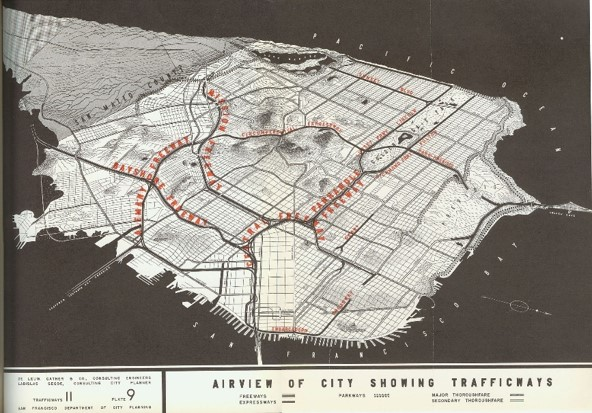
\includegraphics[height=0.3\textheight]{chp01_旧金山.jpg}
%       \caption{1948年旧金山路网规划图}
%     \end{figure}
%   \end{column}
%   \begin{column}{.6\textwidth}
%     \begin{figure}\flushleft
%       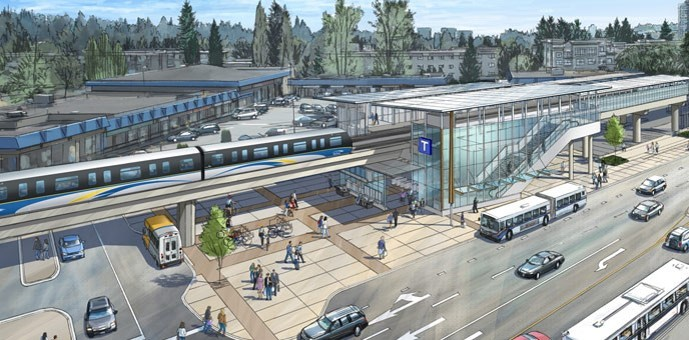
\includegraphics[height=0.3\textheight]{chp01_交通设计.jpg}
%       \caption{城市公交站点交通设计图}
%     \end{figure}
%   \end{column}
% \end{columns}
\begin{figure}\flushright
  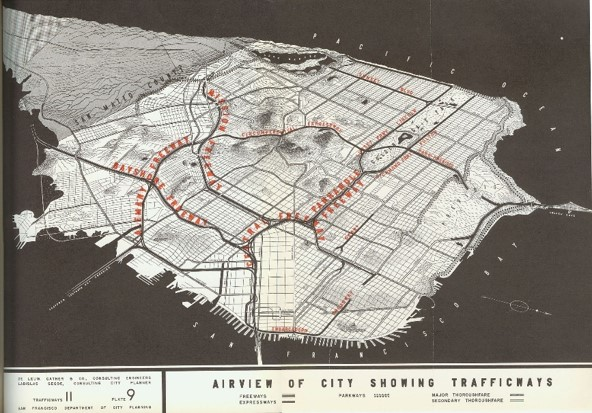
\includegraphics[height=0.7\textheight]{chp01_旧金山.jpg}
  \caption{1948年旧金山路网规划图}
\end{figure}
\end{frame}

\begin{frame}[t]{\subsecname}
\begin{itemize}
\item \emphText{交通调查}是交通规划业务最主要的数据来源,并以此为依据建立分析模型推断规划方案
\item 国内一般\emphText{5--10年}进行一次城市居民出行调查,每次调查的时间长达数月甚至一年
\end{itemize}

\begin{figure}
  \centering
  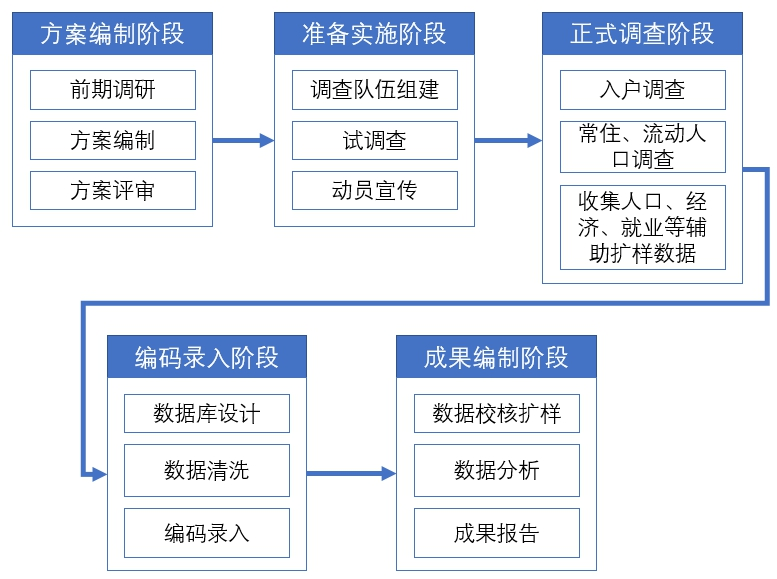
\includegraphics[width=0.65\textwidth]{chp01_交通调查.jpg}
  \caption{交通调查的一般流程}
\end{figure}
\end{frame}

\subsection{什么是大数据}

\begin{frame}[t]{\subsecname}
\begin{goodbox}{IBM公司对大数据的定义}
\begin{enumerate}\footnotesize
    \item Volume:海量的数据规模
    \item Velocity:快速的数据流转和动态的数据体系
    \item Variety:多样的数据类型
    \item Value:巨大的数据价值
    \item Veracity:数据的准确性和可信赖度
\end{enumerate}
\end{goodbox}

\begin{figure}
\begin{columns}
  \begin{column}{.5\textwidth}
      
\includegraphics[height=0.35\textheight]{chp01_文字云.png}
  \end{column}
  \begin{column}{.5\textwidth}
      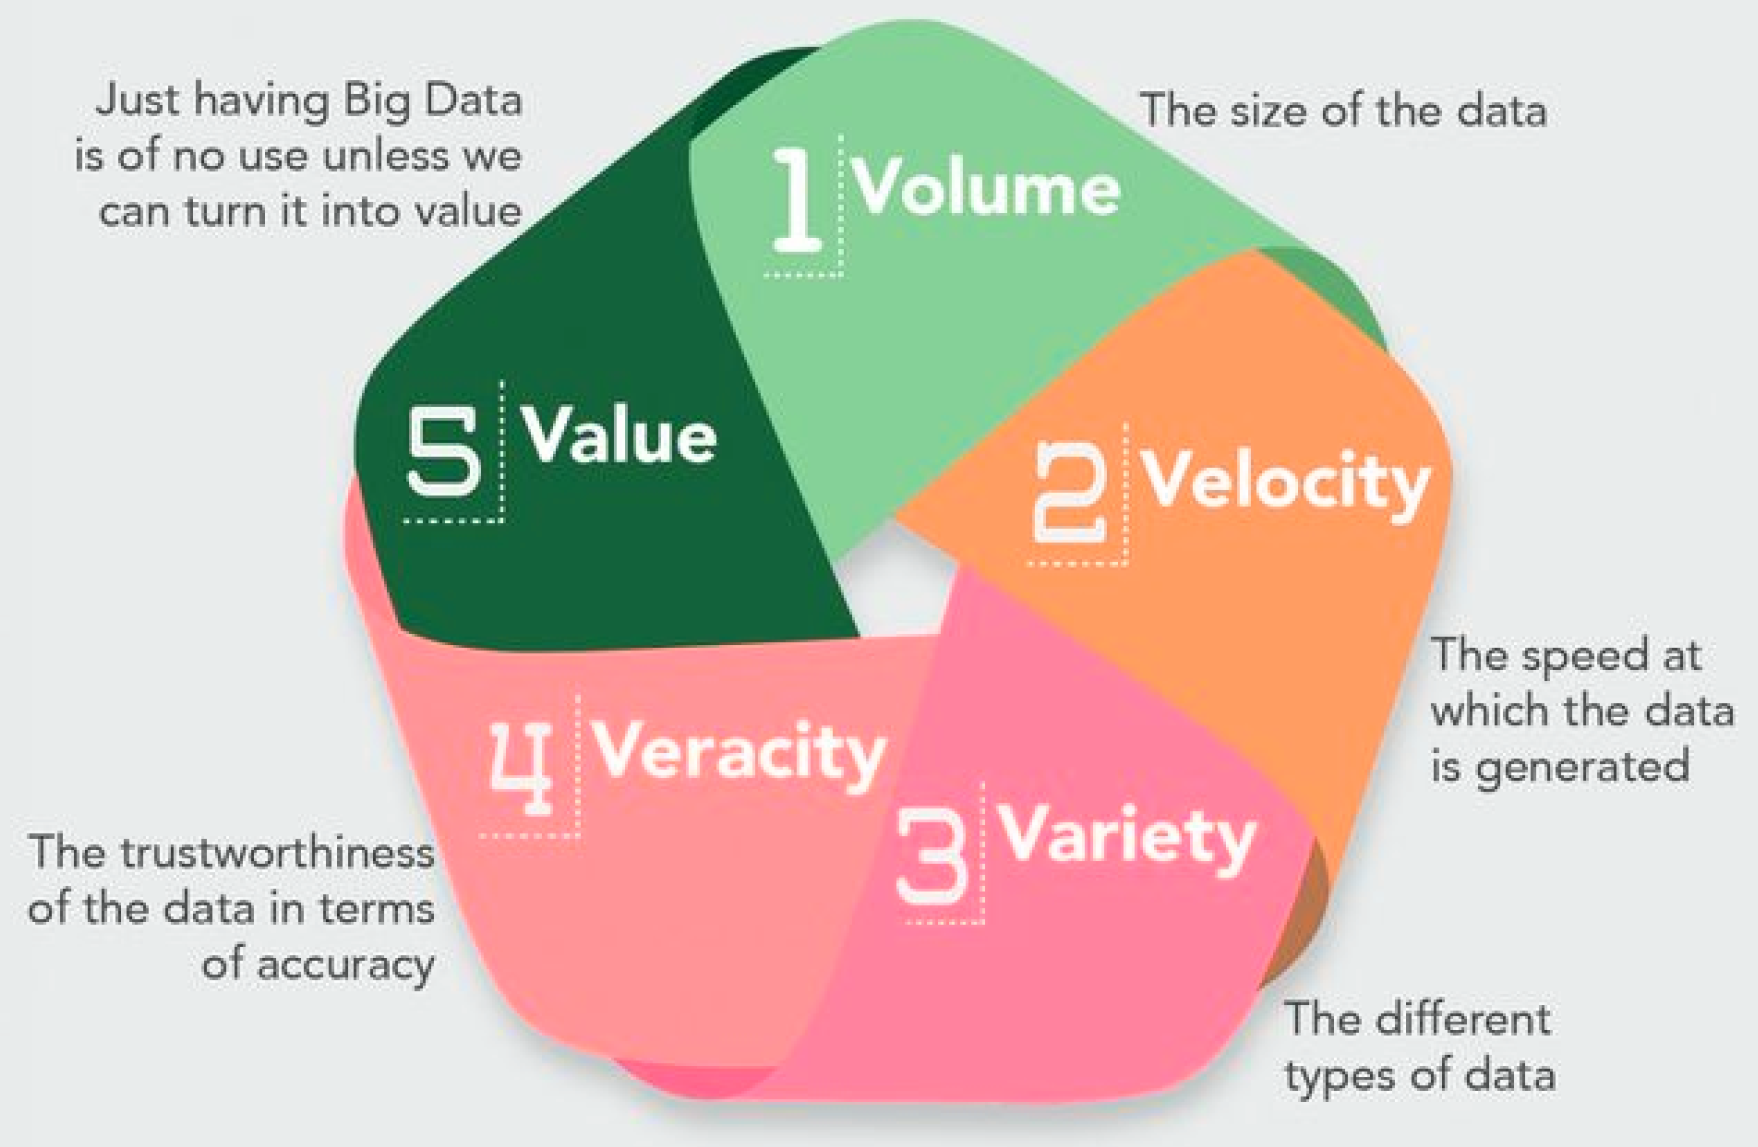
\includegraphics[height=0.35\textheight]{chp01_5V.png}
  \end{column}
\end{columns}
\caption{大数据的5V定义}
\end{figure}
\end{frame}

\begin{frame}[t]{\subsecname}
\begin{itemize}
\item<1-> 与传统数据相比,不仅体现在数据量巨大,更重要的是可以覆盖业务的近乎全部数据
\item<2-> 数据爆炸时代的必然产物
\item<3-> 商业公司进行的一场成功的营销 
\end{itemize}

\begin{overlayarea}{\textwidth}{\textheight}
  \begin{onlyenv}<4>
     \begin{columns}
       \begin{column}{.3\textwidth}
       \begin{figure}
         \centering 
\includegraphics[width=\columnwidth]{chp01_bigdatabook.png}
       \end{figure}
       \end{column}
       \begin{column}{.7\textwidth}
      \begin{ornamentblock}
          \hspace*{2em}大数据是一场思维的颠覆:放弃对因果关系(为什么)的渴求,
而取而代之关注相关关系(是什么)。\\
          \rightline{\textemdash 维克托$\cdot$迈尔$\cdot$舍恩伯格}
      \end{ornamentblock}
       \end{column}
     \end{columns}
  \end{onlyenv}
\end{overlayarea}
\end{frame}

\subsection{大数据对规划编制的意义}

\begin{frame}[t]{\subsecname}
\begin{itemize}
\item<1-> 外部条件与时代背景
\pause
\begin{commonbox}{技术进步} 
随着计算机技术的发展,尤其是云计算和人工智能技术的进步,使得数据获取变得容易了许多,而且处理和分析的能力越来越强
\end{commonbox}
\pause 
\begin{commonbox}{经济转型} 
当前中国的经济正处于重要的转型时期,经济的发展模式、发展要素、发展路径等等都亟需转变,以适应现在的大环境
\end{commonbox}
\pause
\begin{commonbox}{社会转型} 
虽然我们的经济实现了快速发展,但社会矛盾出现越来越尖锐化的趋势
\end{commonbox}
\end{itemize}
\end{frame}

\begin{frame}[t]{\subsecname}
\begin{itemize}
\item 传统城市空间规划面临方法转型
\end{itemize}

\begin{commonbox}{规划转型} 
\begin{itemize} 
\item 传统时空间概念被重新定义,以空间研究和布局为核心内容的城市空间规划
面临着研究范式的转型和规划编制方法上的革新
\item 随着国内城市化进程的发展,规划面临的更多是城市的存量式发展,由粗放向集约进行转型,
对规划的精细化、定量化管理提出了要求
\end{itemize}
\end{commonbox}
\begin{figure}
  \centering
  
\includegraphics[width=0.85\textwidth]{chp01_规划转型.jpg}
  \caption{南京大学规划专业试行的学科教学改革方案}
\end{figure}
\end{frame}

\begin{frame}[t]{\subsecname}
\begin{itemize}
\item 大数据提供了认识和分析城市问题\emphText{新的思维和技术方法}
\item 大数据时代到来,可以让我们更清楚地了解和观察城市的发展、变化过程,同时也\emphText{使得规划过程变得透明可控};
\item 大数据技术强化了对规划过程的重视和科学化,尤其是对规划调研、空间分析、公共参与与空间协调规划、
空间预测和可视化等过程的科学把握,\emphText{有助于推动规划过程的科学化}
\end{itemize}
\begin{figure}
  \centering
  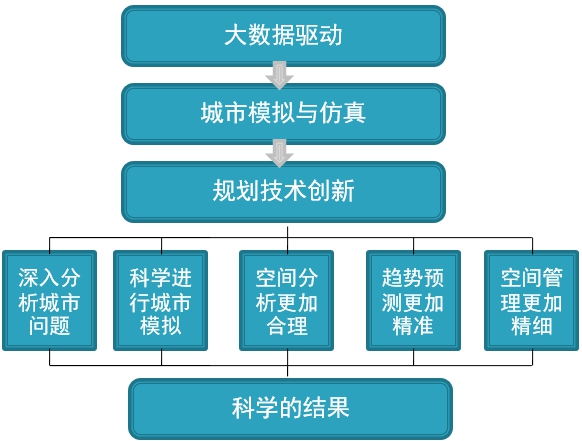
\includegraphics[width=0.55\textwidth]{chp01_数据驱动的城市规划.jpg}
  \caption{大数据驱动的规划决策评估架构}
\end{figure}
\end{frame}
%
%%% Local Variables:
%%% mode: latex
%%% TeX-master: t
%%% End:
%%%%%%%%%%%%%%%%%%%%%%%%%%%%%%%%%%%%%%%%%%%%%%%%%%%%%%%%%%%%

%%%%%%%%%%%%%%%%%%%%%%%%%%%%%%%%%%%%%%%%%%%%%%%%%%%%%%%%%%%%
\section{数据``菜谱''}

\begin{frame}{数据分类}
\begin{itemize}
\item<1-> 地理信息数据
   \begin{enumerate}
     \item 交通网络数据
     \item 土地利用和建筑物数据
     \item 地形图和影像数据
  \end{enumerate}
\item<2-> 静态调查数据
   \begin{enumerate}
     \item 居民出行调查数据
     \item 跨界调查数据
   \end{enumerate}
\item<3-> 动态大数据
   \begin{enumerate}       
       \item 车辆GPS数据
       \item 车牌识别数据
       \item 公交刷卡数据
       \item 手机定位数据
       \item 互联网定位数据
   \end{enumerate}
\item<4-> 互联网开放数据
   \begin{enumerate}
     \item 互联网地图
     \item 交通出行
  \end{enumerate}
\end{itemize}
\end{frame}

\subsection{交通网络数据}
\begin{frame}[t]{\subsecname}
\begin{itemize}
\item<1-> 非结构化网络,用于规划编制成果效果成图
\item<2-> 基于节点-弧段模型的结构化网络,用于定量分析和自动化制图
\end{itemize}

\begin{overlayarea}{\textwidth}{\textheight}
  \begin{onlyenv}<1>
\begin{figure}
  \centering
  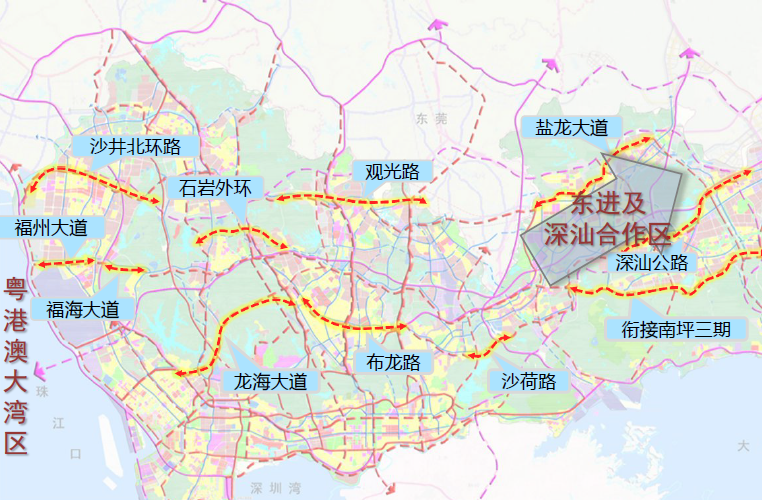
\includegraphics[width=0.8\textwidth]{chp02_非结构化路网.png}
  \caption{规划项目中常用的非结构化网络,无法直接用于定量分析}
\end{figure}
  \end{onlyenv}

  \begin{onlyenv}<2>
\begin{figure}
\begin{columns}
  \begin{column}{.5\textwidth}\centering    
    \begin{tikzpicture}
[intersection/.style={circle,draw=blue!50,fill=blue!20,thick,
inner sep=0pt,minimum size=2mm}]
       \draw[very thick] (-2,0) -- (2,0);
       \draw[very thick] (0,2) -- (0,-2);
       \node at (0,0) [intersection] {};
       \node at (-1,0) [label=below:1]{};
       \node at (1,0) [label=above:2]{};
       \node at (0,1) [label=left:3]{};
       \node at (0,-1) [label=right:4]{}; 
    \end{tikzpicture}
  \end{column}

  \begin{column}{.5\textwidth}\centering \xiaosihao
$
 \left\{
 \begin{matrix}
   0 & 1 & 1 & 1 \\
   1 & 0 & 1 & 1 \\
   1 & 1 & 0 & 1 \\
   1 & 1 & 1 & 0  
  \end{matrix}
  \right\} 
$
  \end{column}
\end{columns}
\caption{交通网络在计算机中的结构化存储形式}
\end{figure}
  \end{onlyenv}
\end{overlayarea}
\end{frame}

\begin{frame}[t]{\subsecname}
\begin{itemize}
\item<1-> 道路网络,共 路段,多少节点   
\item<3-> 轨道网络
\item<4-> 公交网络
\end{itemize}

\begin{overlayarea}{\textwidth}{\textheight}
  \begin{onlyenv}<1>
\begin{figure}\centering
    \subfloat[百度地图]
    {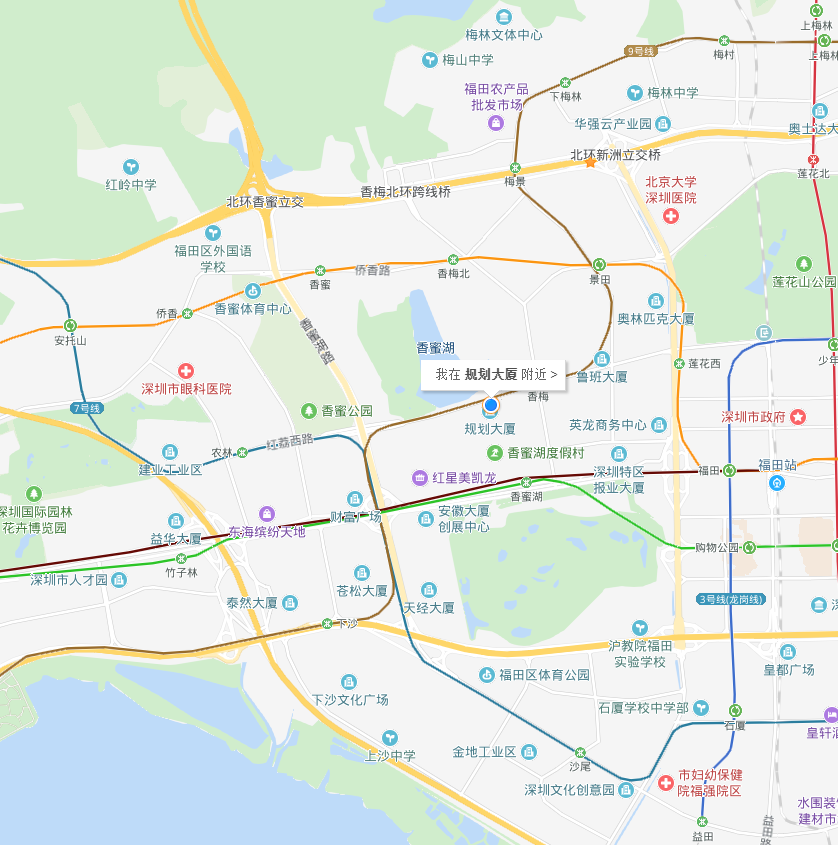
\includegraphics[height=0.5\textheight]{chp02_百度地图.png}}\vspace{1pt} 
    \subfloat[openstreetmap地图]
    {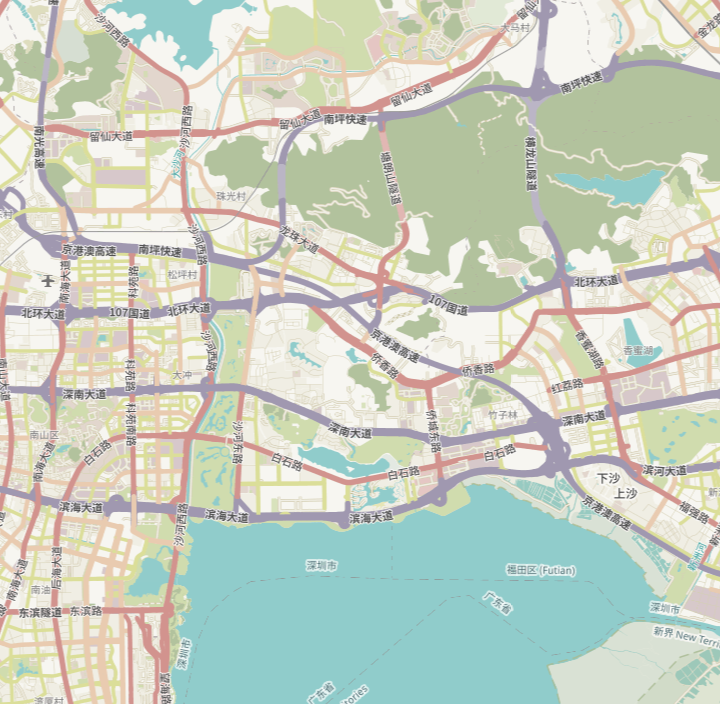
\includegraphics[height=0.5\textheight]{chp02_OSM.png}}
    \caption{互联网地图中基于结构化数据的自动化制图技术}
\end{figure}
  \end{onlyenv}

  \begin{onlyenv}<2>
\begin{table} \centering \scriptsize
  \renewcommand\arraystretch{0.9}
  \begin{tabular}{|m{0.3\columnwidth}|m{0.3\columnwidth}|m{0.3\columnwidth}|}
    \toprule
    \rowcolor{LightCyan}
\multicolumn{1}{|c|}{\textbf{属性名称}} & \multicolumn{1}{c|}{\textbf{含义}} & \multicolumn{1}{c|}{\textbf{类型}}\\\hline
    NAME & 道路名称 & 字符型 \\\hline
    CDS & 车道数 & 整数型 \\\hline
    LEN & 道路长度 & 浮点型 \\\hline
    LDKD & 道路宽度 & 浮点型 \\\hline
    FJDCDKD & 非机动车道宽度 & 浮点型 \\\hline
    JDCDKD & 机动车道宽度 & 浮点型 \\\hline
    RXDKD & 人行道宽度 & 浮点型 \\\hline
    HXKD & 红线宽度 & 浮点型 \\\hline
    DLDJ & 道路等级 & 整数型 \\\hline
    JTXTJ & 可通行交通方式 & 字符型 \\\hline
    GJZYD & 是否具备公交专用道 & 布尔型 \\
    \bottomrule
  \end{tabular}
\caption{道路网络包含的主要属性信息}
\end{table}
  \end{onlyenv}
\end{overlayarea}

\end{frame}

\subsection{土地利用和建筑物数据}
\begin{frame}[t]{\subsecname}
\begin{itemize}
\item 规土委核心数据,一张图系统提供
\end{itemize}

\begin{overlayarea}{\textwidth}{\textheight}
\vspace{-5pt}
  \begin{onlyenv}<1>
\begin{figure}
  \centering
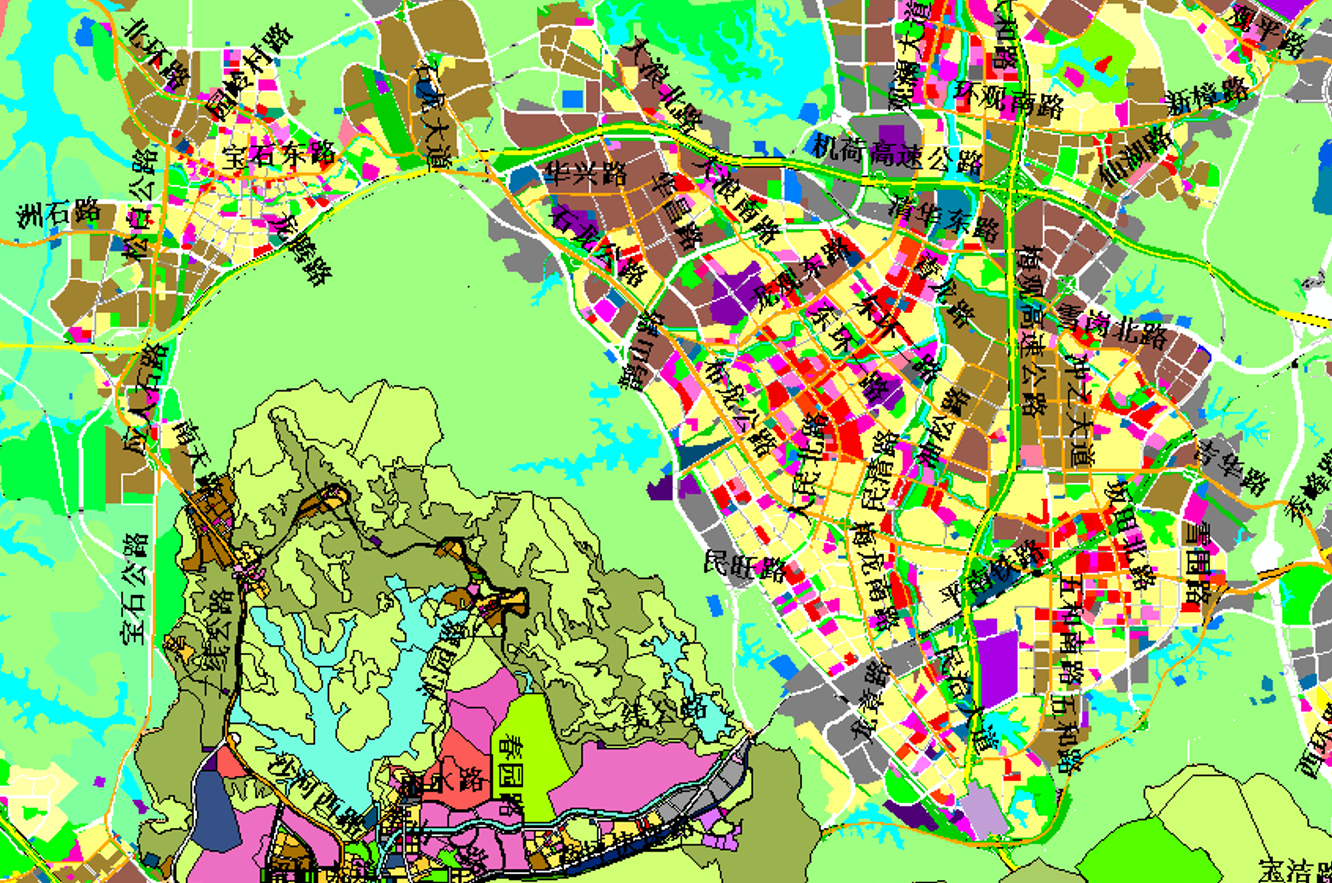
\includegraphics[width=0.9\textwidth]{chp02_土地利用.png}
  \caption{土地利用数据}
\end{figure}
  \end{onlyenv}

\vspace{-5pt}
  \begin{onlyenv}<2>
\begin{figure}
  \centering
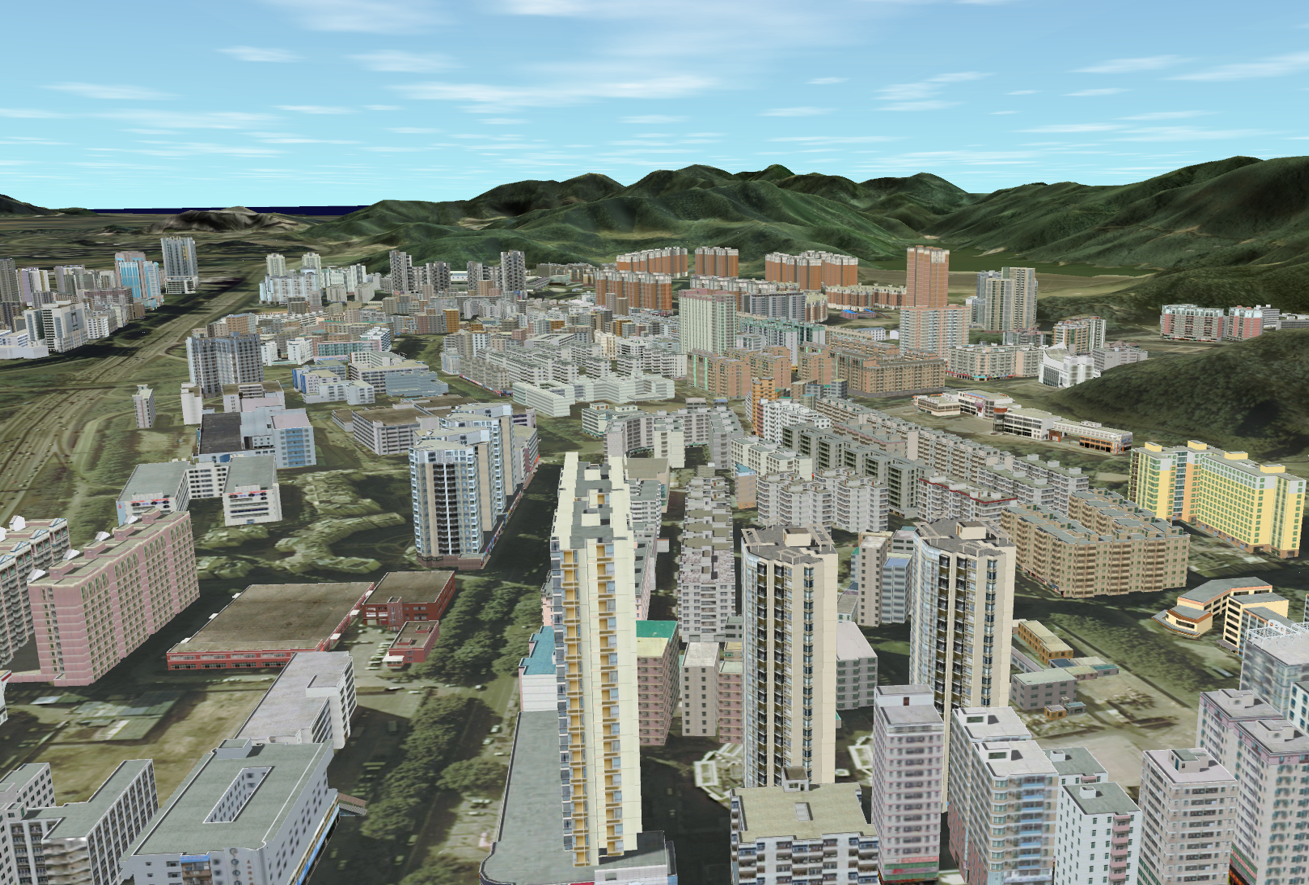
\includegraphics[width=0.9\textwidth]{chp02_建筑物.png}
  \caption{建筑物数据}
\end{figure}
  \end{onlyenv}
\end{overlayarea}
\end{frame}

\subsection{地形图和影像数据}

\begin{frame}[t]{\subsecname}
\begin{itemize}
\item 规土委涉密数据,向信息中心申请 
\end{itemize}

\begin{overlayarea}{\textwidth}{\textheight}
\vspace{-5pt}
  \begin{onlyenv}<1>
\begin{figure}
  \centering
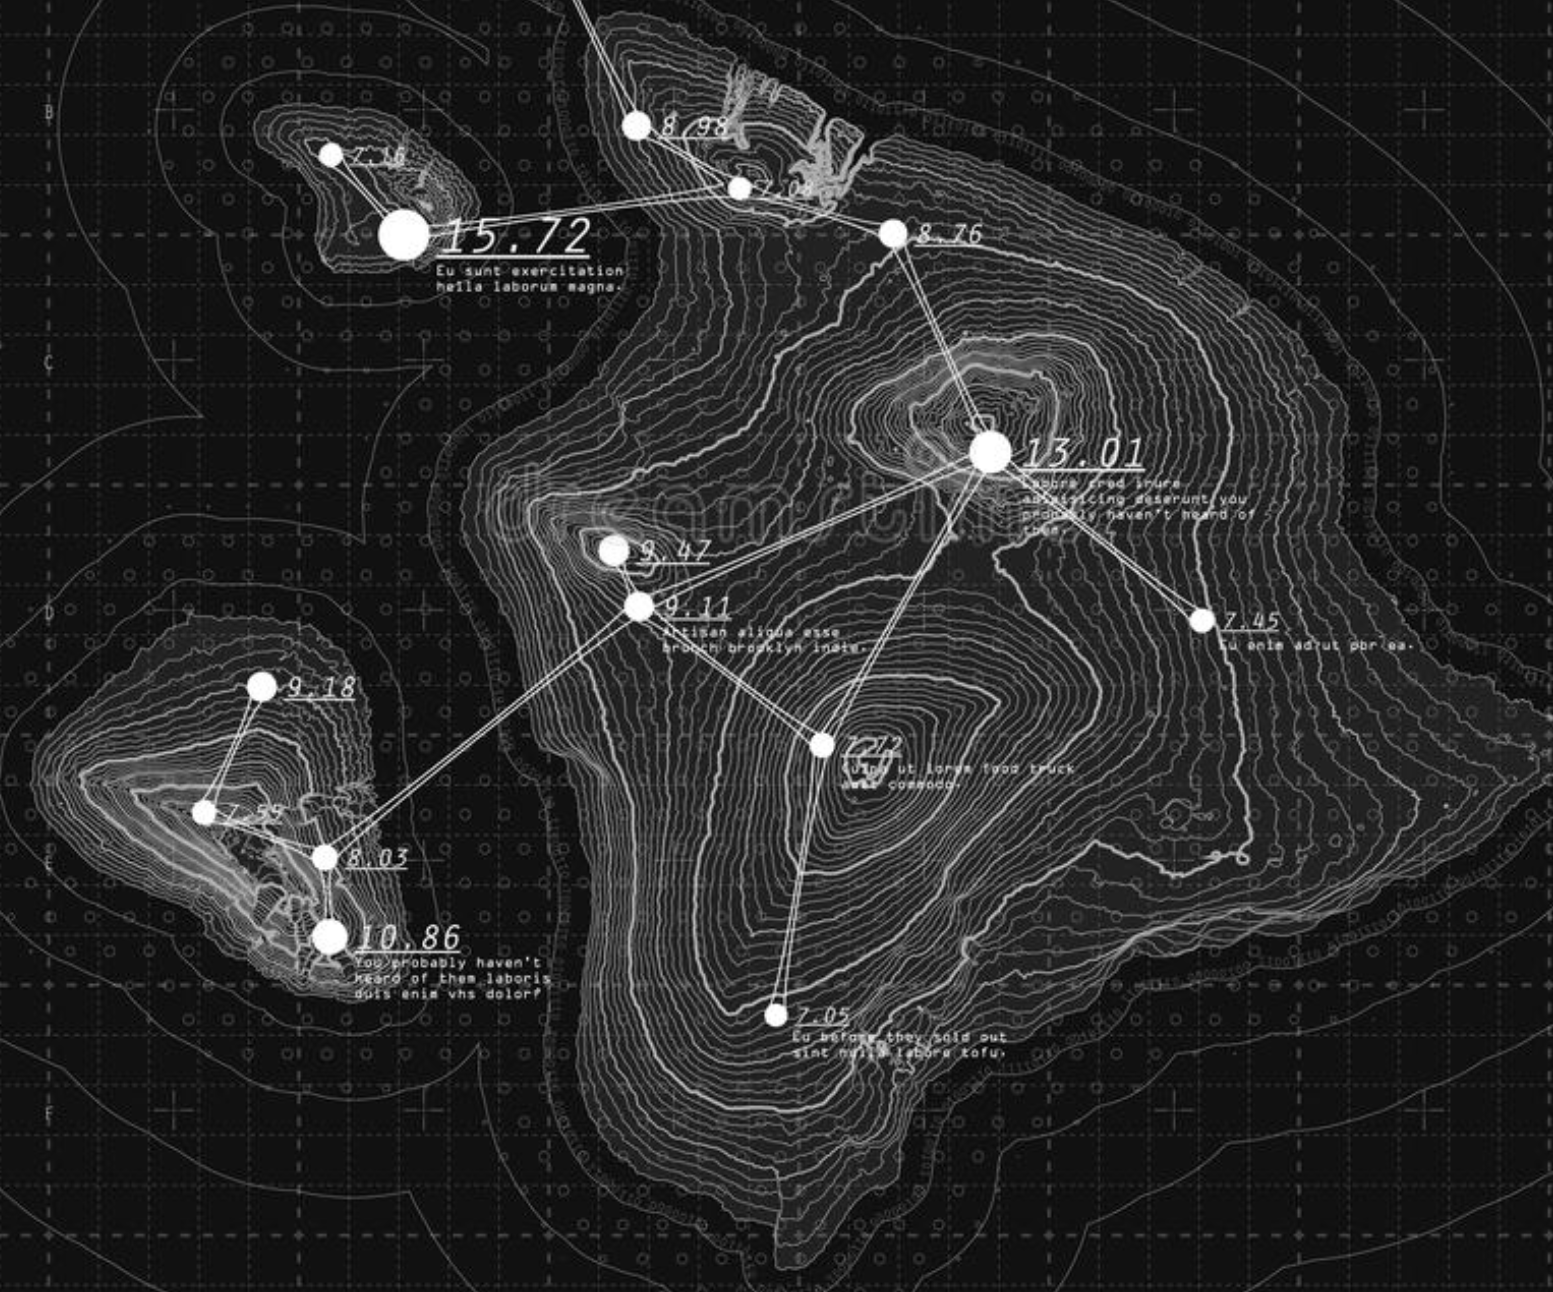
\includegraphics[width=0.75\textwidth]{chp02_地形图.png}
  \caption{地形图数据}
\end{figure}
  \end{onlyenv}

\vspace{-10pt}
  \begin{onlyenv}<2>
\begin{figure}
  \centering
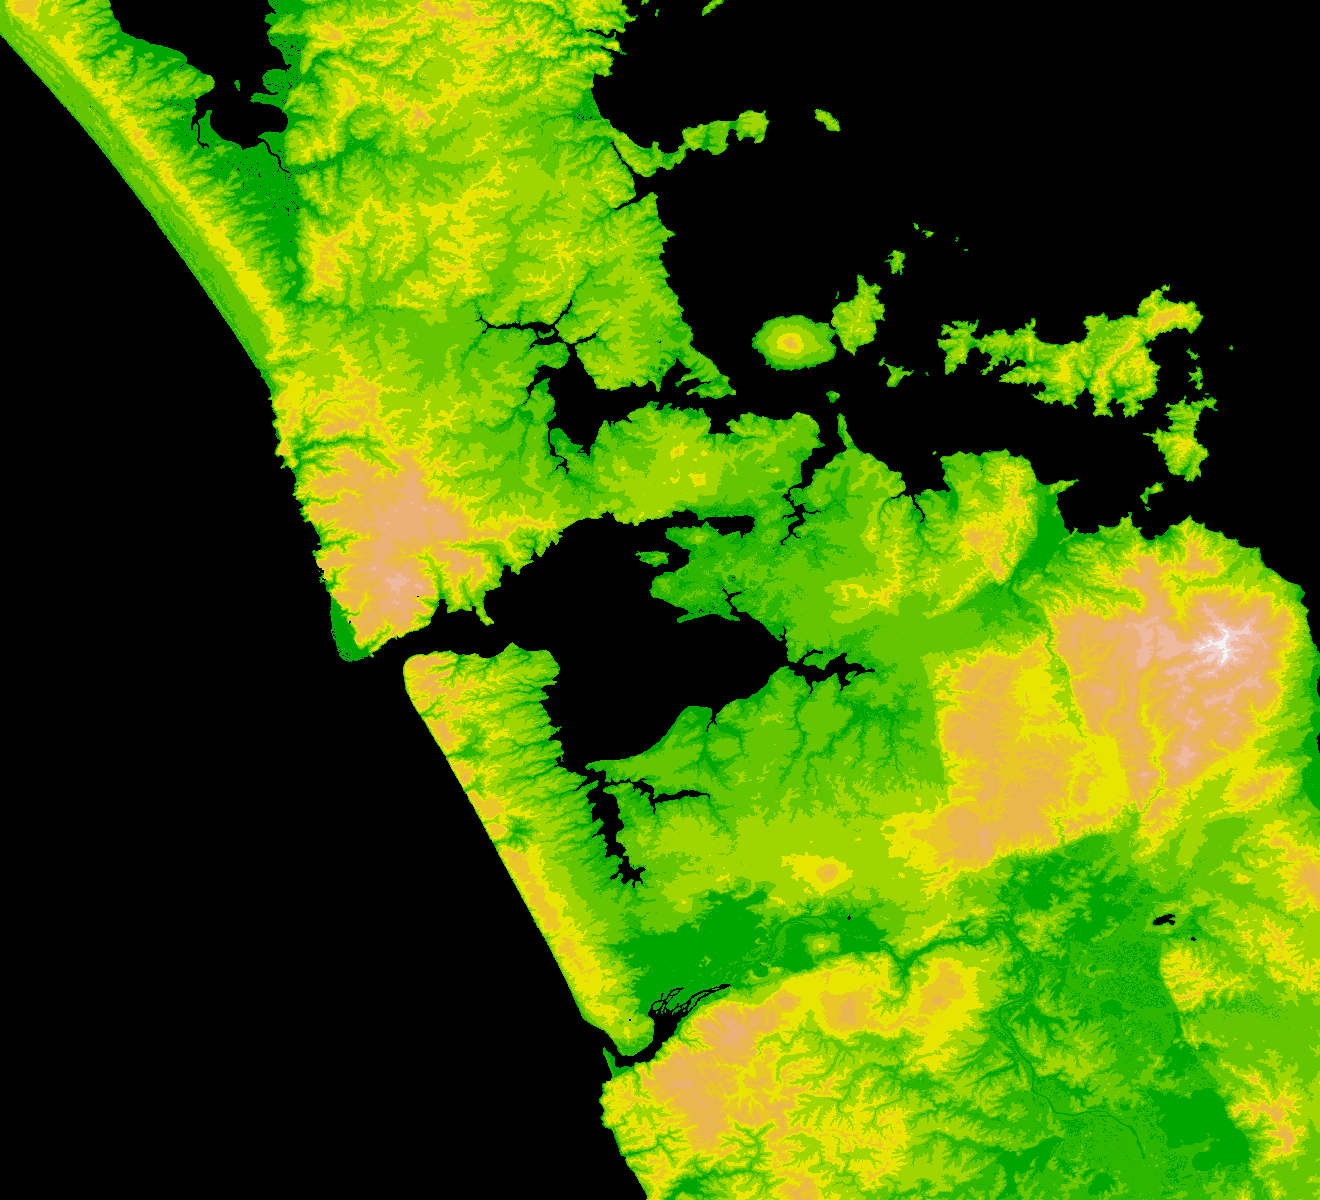
\includegraphics[width=0.7\textwidth]{chp02_遥感影像.png}
  \caption{遥感影像数据}
\end{figure}
  \end{onlyenv}
\end{overlayarea}
\end{frame}


\subsection{居民出行调查数据}

\begin{frame}[t]{\subsecname}
\begin{itemize}
\item<2-> 2005、2010、2016三次居民出行调查数据
\item<3-> 最终数据成果是\emphText{户表、人表和出行表}共三张表
\end{itemize}

\begin{overlayarea}{\textwidth}{\textheight}
  \begin{onlyenv}<2>
\begin{figure}
  \centering
  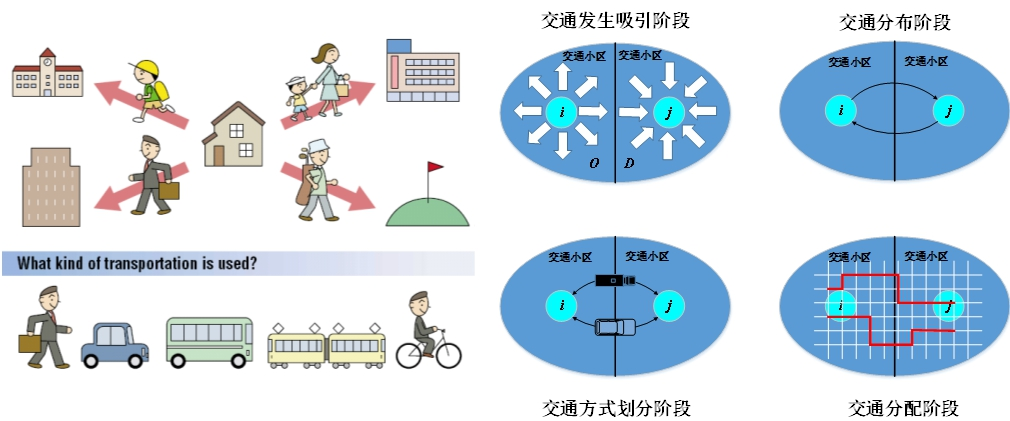
\includegraphics[width=\textwidth]{chp01_居民出行调查.jpg}
  \caption{以家庭为单位,调查家庭成员出行次数、出行目的、交通方式和目的地}
\end{figure}
  \end{onlyenv}

\begin{onlyenv}<3>
  \begin{table} \centering \footnotesize
    \begin{tabular}{|>{\centering\arraybackslash} m{0.15\columnwidth}|m{0.7\columnwidth}|}
      \toprule
      \rowcolor{LightCyan}
      \multicolumn{1}{|c|}{\textbf{主要字段}} & \multicolumn{1}{c|}{\textbf{说明}} \\\hline
      户ID & 唯一值\\\hline
      回答时间 & 填写问卷的时间\\\hline
      建筑物位置 & 被访问者居住地,经纬度坐标\\\hline
      户类型 & 家庭户:1;集体户:2\\\hline
      居住人数 & 分为$\geq{4}$岁人数和$<4$岁人数\\\hline
      家庭年收入 & $\leq{4}$万:1;10-20万:2;20-30万:3;30-50万:4;$\geq{50}$万:5\\\hline
      住房来源 & 租赁廉租房、租赁城中村、租赁其他住房、自建房、购买商品房、购买福利房或保障房、集体宿舍\\\hline
      拥车情况 & 是否拥有小汽车?家庭拥有几辆小汽车?\\\hline
      \bottomrule
    \end{tabular}
    \caption{户表}
  \end{table}
\end{onlyenv}

\begin{onlyenv}<4>
  \begin{table} \centering \footnotesize
    \begin{tabular}{|>{\centering\arraybackslash} m{0.15\columnwidth}|m{0.7\columnwidth}|}
      \toprule
      \rowcolor{LightCyan}
      \multicolumn{1}{|c|}{\textbf{主要字段}} & \multicolumn{1}{c|}{\textbf{说明}} \\\hline
      人ID & 与户ID对应\\\hline
      年龄 & \\\hline
      性别 & \\\hline
      户口登记情况 & 本市户籍:1;非本市户籍:2。其中,非本市户籍中是否居住6个月以上\\\hline
      文化程度 & 分为9个选项\\\hline
      职业 & 分为9个选项\\\hline
      所属行业 & 参考经济普查问卷,分为18个选项\\\hline
      工作地或学校地址 & \\\hline
      \bottomrule
    \end{tabular}
    \caption{人表}
  \end{table}
\end{onlyenv}

\begin{onlyenv}<5>
  \begin{table} \centering \footnotesize
    \begin{tabular}{|>{\centering\arraybackslash} m{0.4\columnwidth}|m{0.5\columnwidth}|}
      \toprule
      \rowcolor{LightCyan}
      \multicolumn{1}{|c|}{\textbf{主要字段}} & \multicolumn{1}{c|}{\textbf{说明}} \\\hline
      出行ID & 与人ID对应\\\hline
      出行和换乘方式 & 公交、小汽车、地铁等共12类\\\hline
      出行目的 & 上班、上学、公务等10类\\\hline
      出发时间 & \\\hline
      出发地点 & 详细地址及经纬度\\\hline
      到达时间 & \\\hline
      到达地点 & 详细地址及经纬度\\\hline
      换乘站点 & \\\hline
      步行时间、候车时间、车内时间 & 公共交通出行 \\\hline
      \bottomrule
    \end{tabular}
    \caption{出行表}
  \end{table}
\end{onlyenv}
\end{overlayarea}
\end{frame}

\subsection{跨界调查数据}

\begin{frame}[t]{\subsecname}
\begin{itemize}
\item 从2013年开始,每两年开展一次跨界客流调查
\item 调查范围包括深圳和东莞、惠州的边界、深圳出境口岸和重要对外交通枢纽
\end{itemize}

\begin{overlayarea}{\textwidth}{\textheight}
  \begin{onlyenv}<2>
\begin{figure}
  \centering
  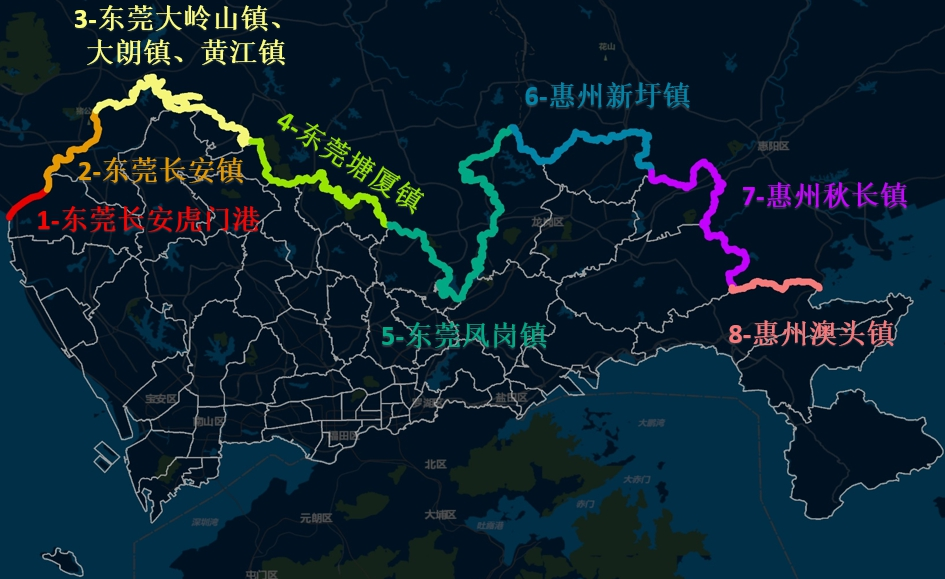
\includegraphics[width=0.85\textwidth]{chp02_境界线.jpg}
  \caption{深莞惠境界线}
\end{figure}
  \end{onlyenv}

  \begin{onlyenv}<3>
\begin{figure}
  \centering
  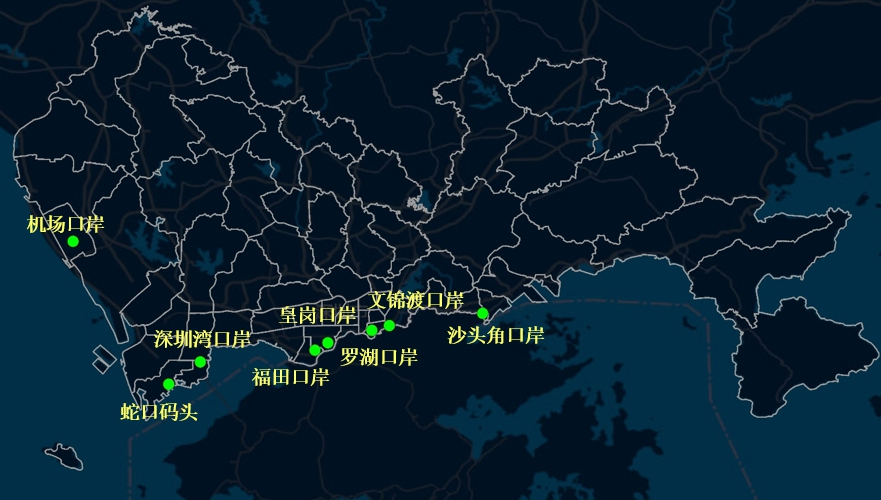
\includegraphics[width=0.85\textwidth]{chp02_口岸.jpg}
  \caption{深港口岸}
\end{figure}
  \end{onlyenv}

  \begin{onlyenv}<4>
\begin{figure}
  \centering
  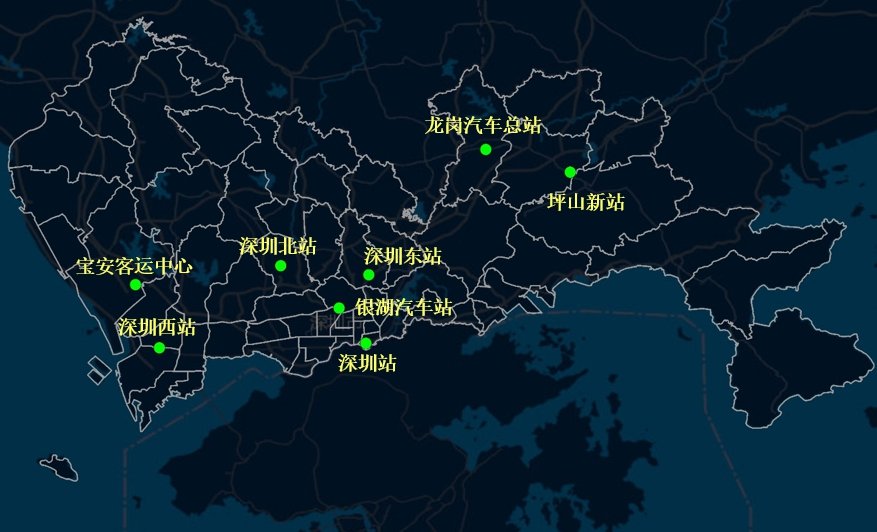
\includegraphics[width=0.8\textwidth]{chp02_交通枢纽.jpg}
  \caption{重要对外交通枢纽}
\end{figure}
  \end{onlyenv}
\end{overlayarea}
\end{frame}

\subsection{车辆GPS数据}

\begin{frame}[t]{\subsecname}
\begin{itemize}
\item<1-> 利用GPS卫星定位车辆,记录车辆位置、时间、方向、速度和状态等信息
\item<1-> 覆盖全部出租车、公交车、特种车以及部分货车,约10万辆
\item<2-> 从2013年开始收集,10-40秒回传一次数据,日均数据量约10GB左右,超过1亿条 
\end{itemize}

\begin{overlayarea}{\textwidth}{\textheight}

  \begin{onlyenv}<1>
\begin{figure}
  \centering
  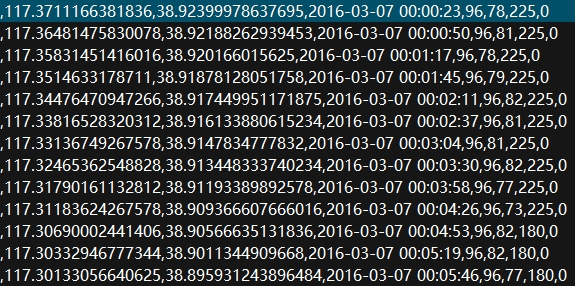
\includegraphics[width=0.85\textwidth]{chp02_GPS原始数据.jpg}
  \caption{GPS原始数据文件,每辆车存储一个文件}
\end{figure}
  \end{onlyenv}

\vspace{-15pt}
  \begin{onlyenv}<2>
\begin{figure}
  \centering
  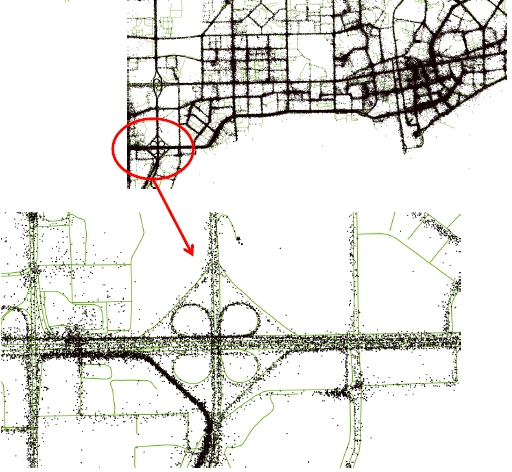
\includegraphics[width=0.5\textwidth]{chp02_空间上的GPS数据.jpg}
  \caption{空间中的GPS数据}
\end{figure}
  \end{onlyenv}

\vspace{5pt}
  \begin{onlyenv}<3>
\begin{figure}
  \centering
  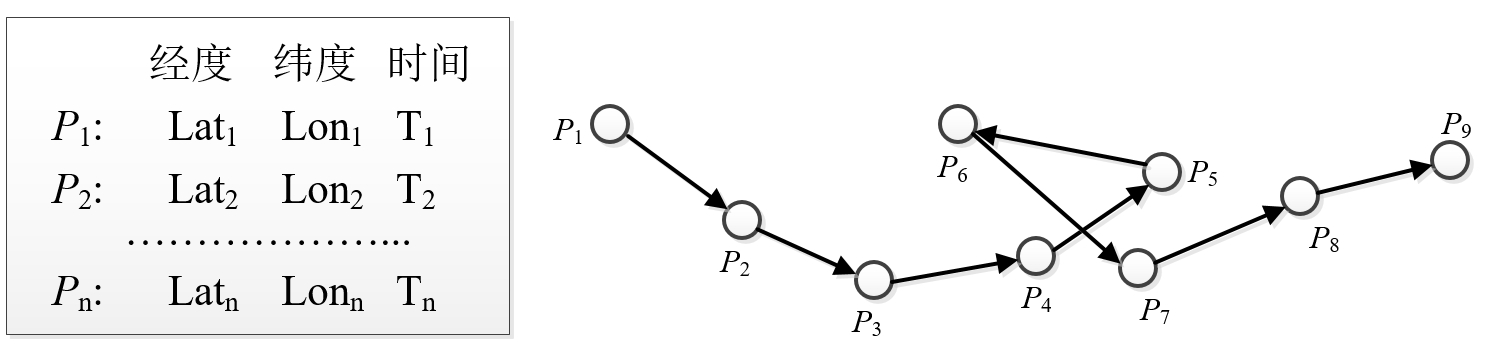
\includegraphics[width=\textwidth]{chp02_GPS示意图.jpg}
  \caption{GPS轨迹数据示意图}
\end{figure}
  \end{onlyenv}

\end{overlayarea}
\end{frame}

\subsection{车牌识别数据}

\begin{frame}[t]{\subsecname}
\begin{itemize}
\item<1-> 通过车牌识别算法,从布设在道路上的拍摄视频中提取车牌
\item<2-> 全市目前有300多个检测点位
\item<2-> 从2014年开始收集,日均数据量是约2.5GB,超过1200万条 
\end{itemize}

%\begin{overlayarea}{\textwidth}{\textheight}

%\vspace{15pt}
\begin{onlyenv}<1>
\begin{figure} \centering
\begin{columns}[b]
  \begin{column}{.5\textwidth}
    \begin{figure}\flushright
      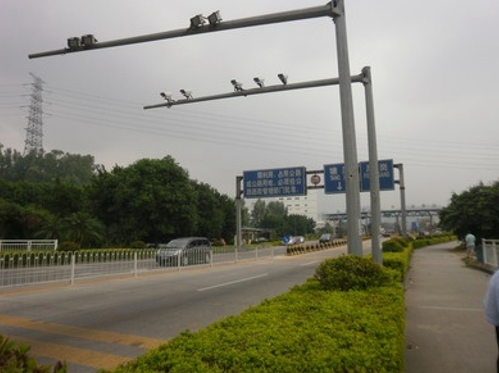
\includegraphics[height=0.35\textheight]{chp02_车牌识别01.jpg}
    \end{figure}
  \end{column}
  \begin{column}{.5\textwidth}
    \begin{figure}\flushleft
      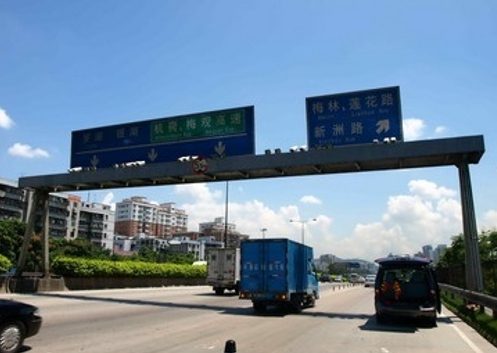
\includegraphics[height=0.35\textheight]{chp02_车牌识别02.jpg}
    \end{figure}
  \end{column}
\end{columns}
\caption{道路上的车辆拍摄设备} 
\end{figure}
\end{onlyenv}
%\end{overlayarea}

\end{frame}

\subsection{公交刷卡数据}

\begin{frame}[t]{\subsecname}
\begin{itemize}
\item<1-> 全部深圳通刷卡数据,包括地铁和常规公交
\item<1-> 包含刷卡时间、终端编号、卡号等信息
\item<2-> 从2013年开始收集,日均数据量3.5GB,超过1500万条
\end{itemize}

\begin{overlayarea}{\textwidth}{\textheight}
  \begin{onlyenv}<1>
\begin{figure} \centering
\begin{columns}[b]
  \begin{column}{.5\textwidth}
    \begin{figure}\flushright
      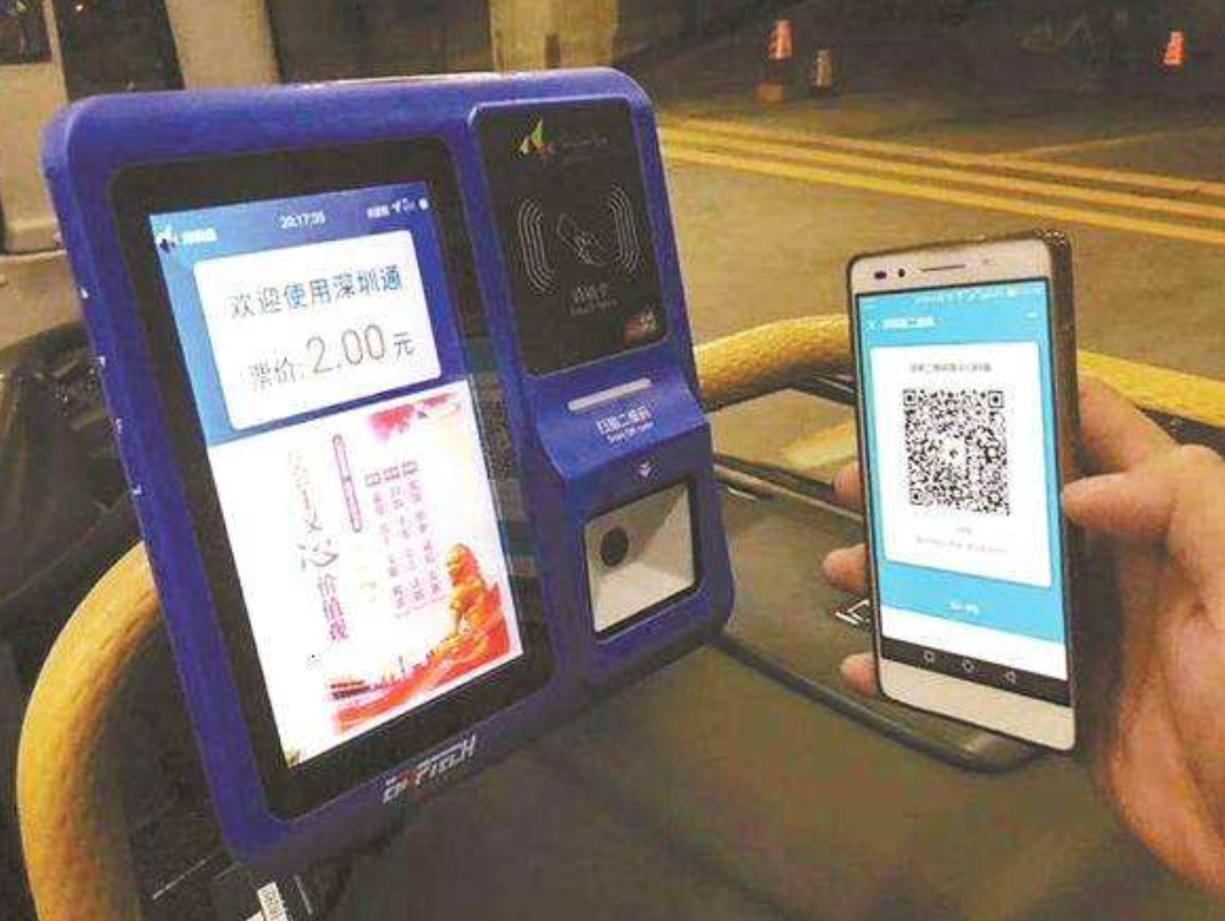
\includegraphics[height=0.4\textheight]{chp02_常规公交刷卡.png}
    \end{figure}
  \end{column}
  \begin{column}{.5\textwidth}
    \begin{figure}\flushleft
      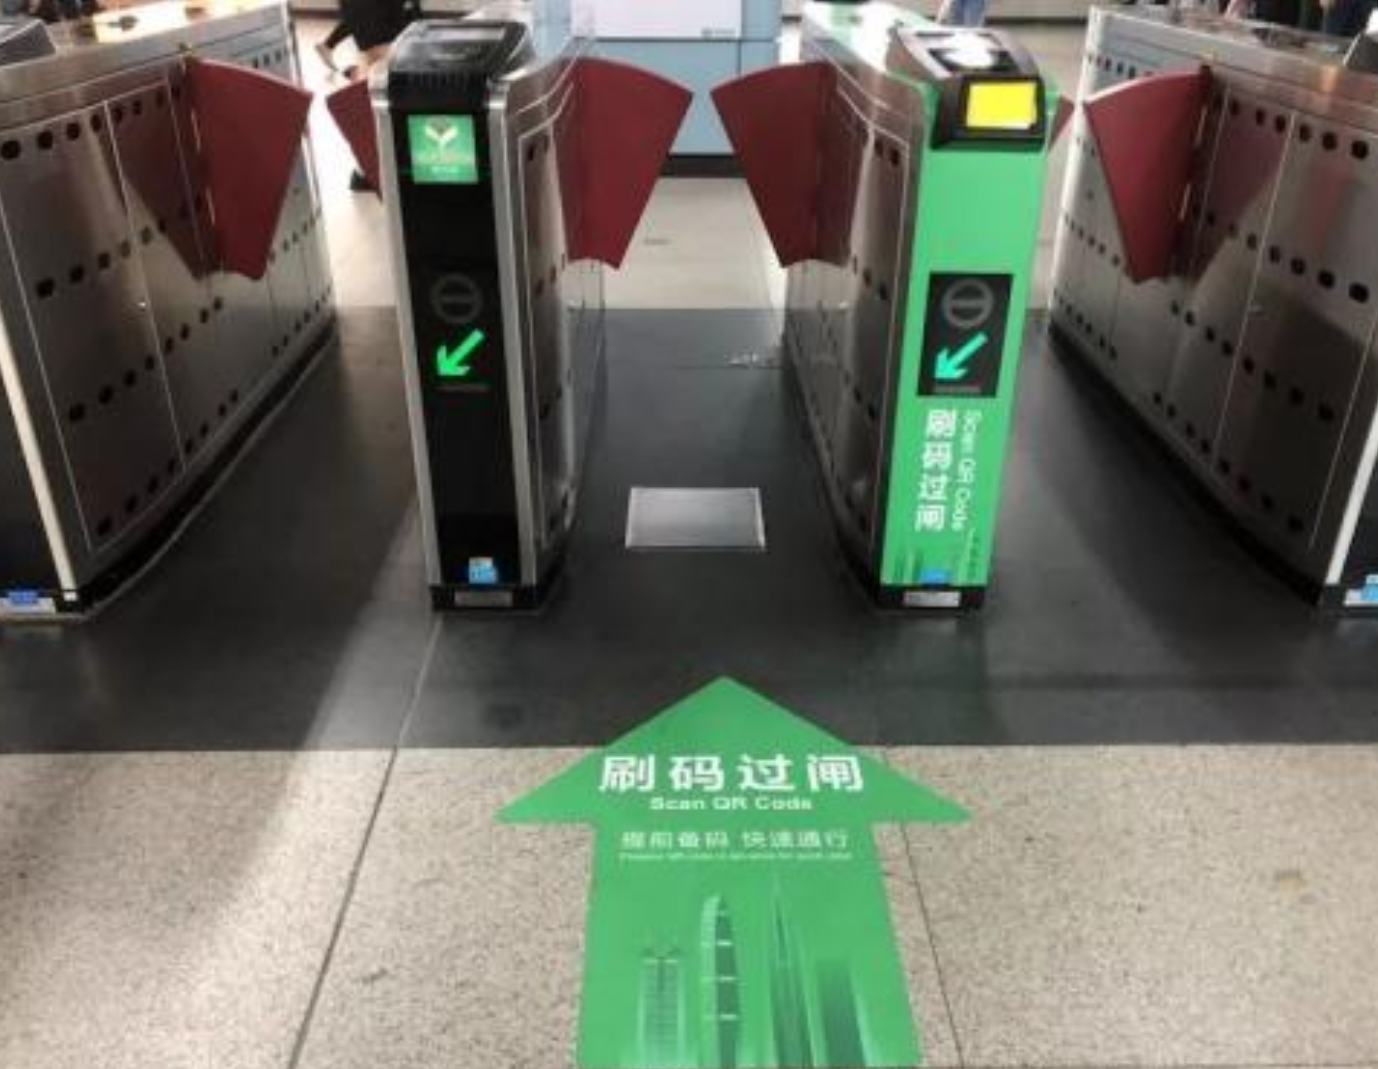
\includegraphics[height=0.4\textheight]{chp02_地铁刷卡.png}
    \end{figure}
  \end{column}
\end{columns}
\caption{深圳通刷卡设备} 
\end{figure}
  \end{onlyenv}
\end{overlayarea}
\end{frame}

\subsection{手机定位数据}
 
\begin{frame}[t]{\subsecname}
\begin{itemize}
\item<1-> 利用手机与基站的通信定位手机位置、时间信息;另外,运营商还掌握机主实名信息
\item<2-> 数据量受采样频率影响,深圳市日均通常可以达到TB级别
\item<2-> 目前只有电信和联通少量处理后的数据
\end{itemize}

\begin{overlayarea}{\textwidth}{\textheight}
\vspace{-5pt}
  \begin{onlyenv}<1>
\begin{figure}
  \centering
  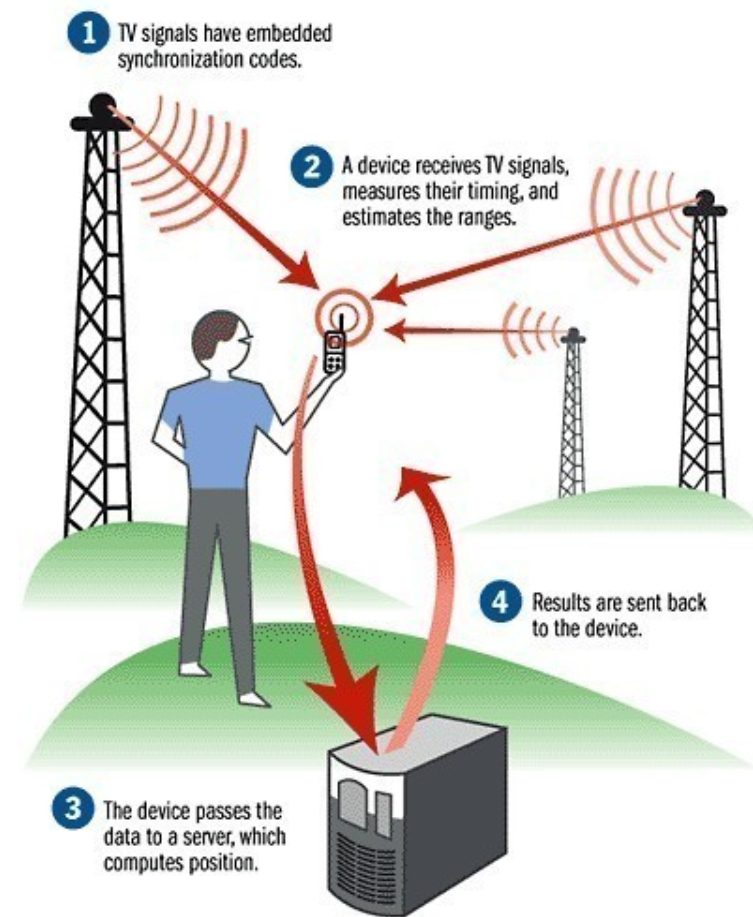
\includegraphics[width=0.4\textwidth]{chp02_手机定位原理.png}
  \caption{手机定位原理}
\end{figure}
  \end{onlyenv}
\end{overlayarea}
\end{frame}

\subsection{互联网定位数据}

\begin{frame}[t]{\subsecname}
\begin{itemize}
\item 利用网络路由、手机GPS等融合技术获取定位信息,由各大互联网公司掌握
\item 互联网公司核心的大数据资源之一,不直接对外开放
\end{itemize}

\begin{figure}\centering
    \captionsetup[subfigure]{labelformat=empty}
    \subfloat[百度利用定位数据制作热力图]
    {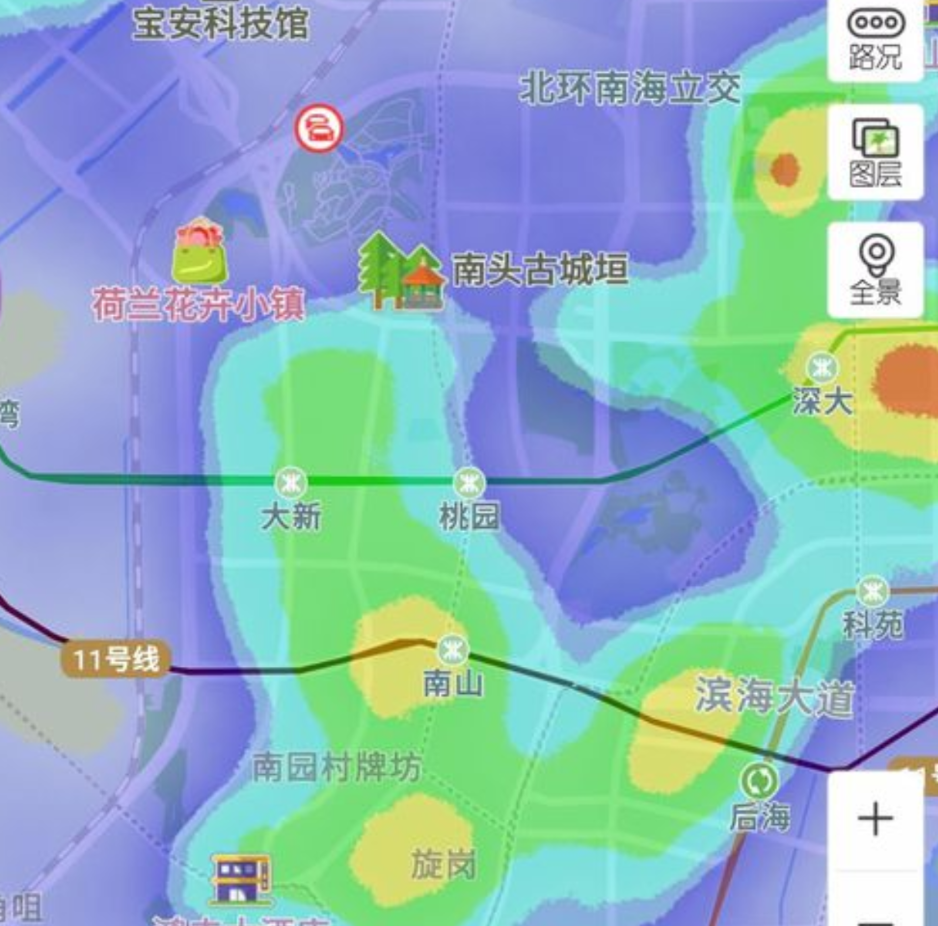
\includegraphics[height=0.45\textheight]{chp02_百度定位数据.png}}\vspace{1pt} 
    \subfloat[腾讯实时定位数据分布]
    {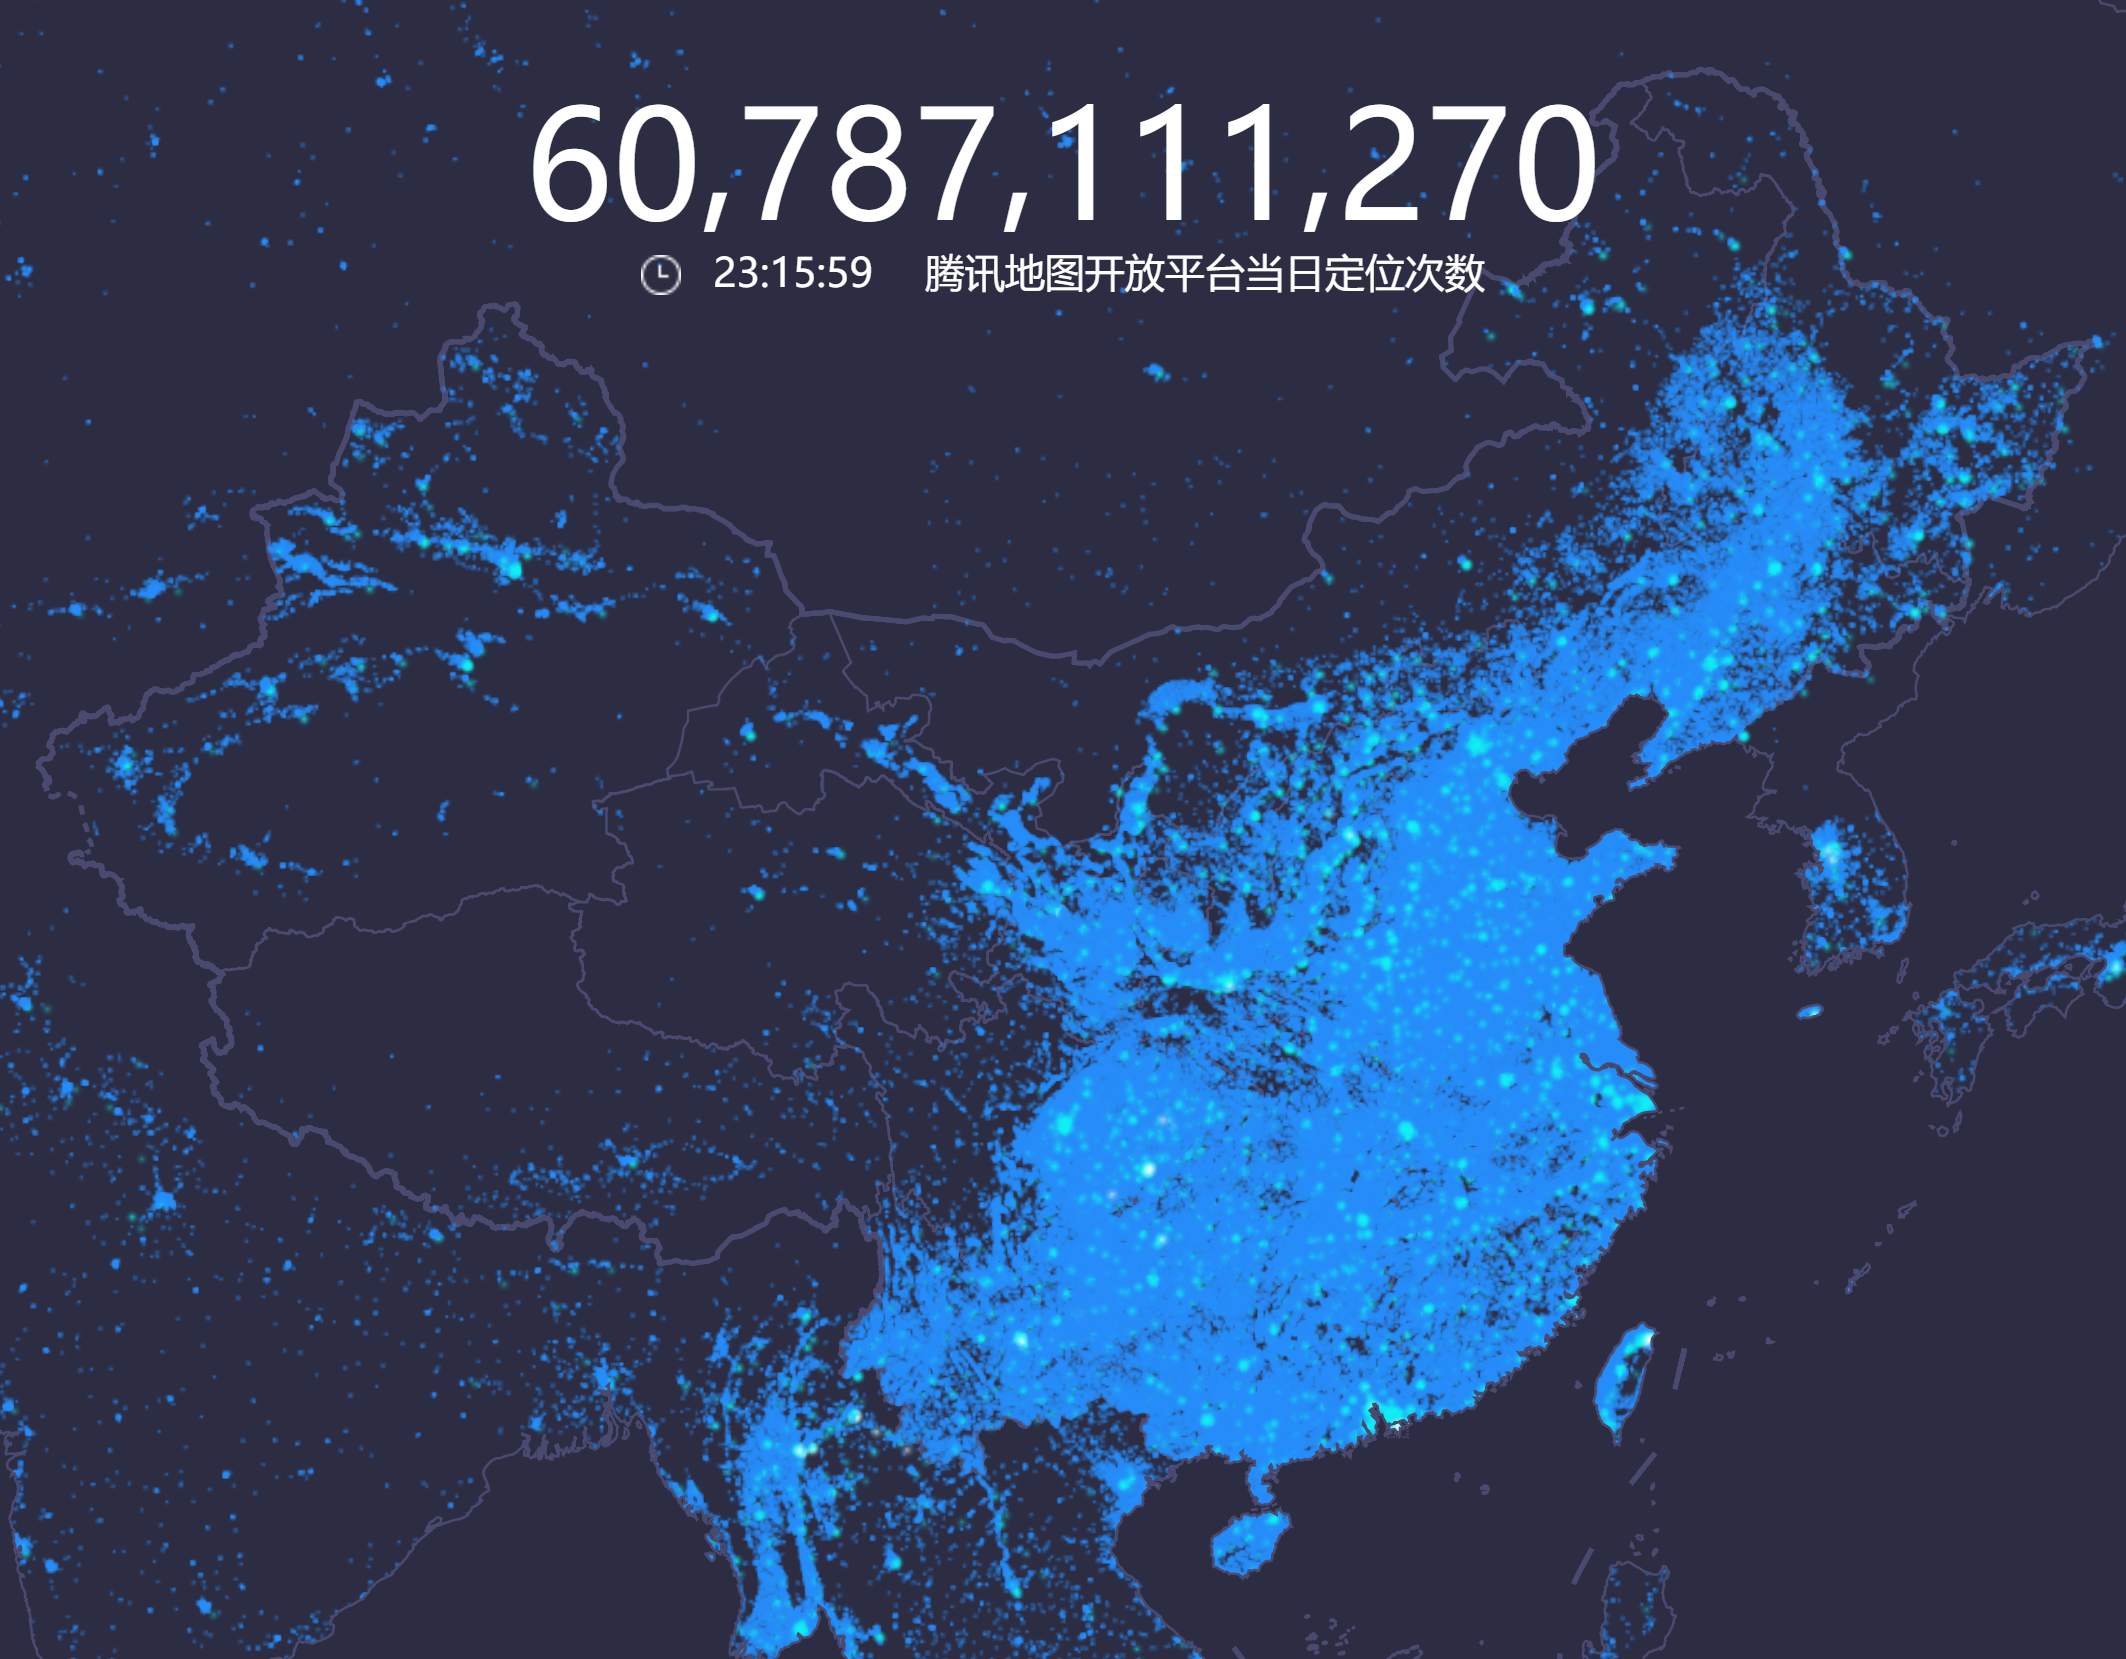
\includegraphics[height=0.45\textheight]{chp02_腾讯定位数据.png}}
\end{figure}
\end{frame}

\subsection{互联网地图}
\begin{frame}[t]{\subsecname}
  \begin{columns}[T]
     \begin{column}[T]{0.5\textwidth}
     \begin{itemize}
        \item<1-> 卫星遥感影像地图
        \item<2-> 制图综合后的瓦片地图
     \end{itemize} \end{column}

     \begin{column}[T]{0.5\textwidth}
     \begin{itemize}
        \item<3-> 兴趣点(POI)数据
        \item<4-> 矢量GIS数据
     \end{itemize} \end{column}
  \end{columns}

\begin{overlayarea}{\textwidth}{\textheight}
  \begin{onlyenv}<1>
\begin{figure}
  \centering
  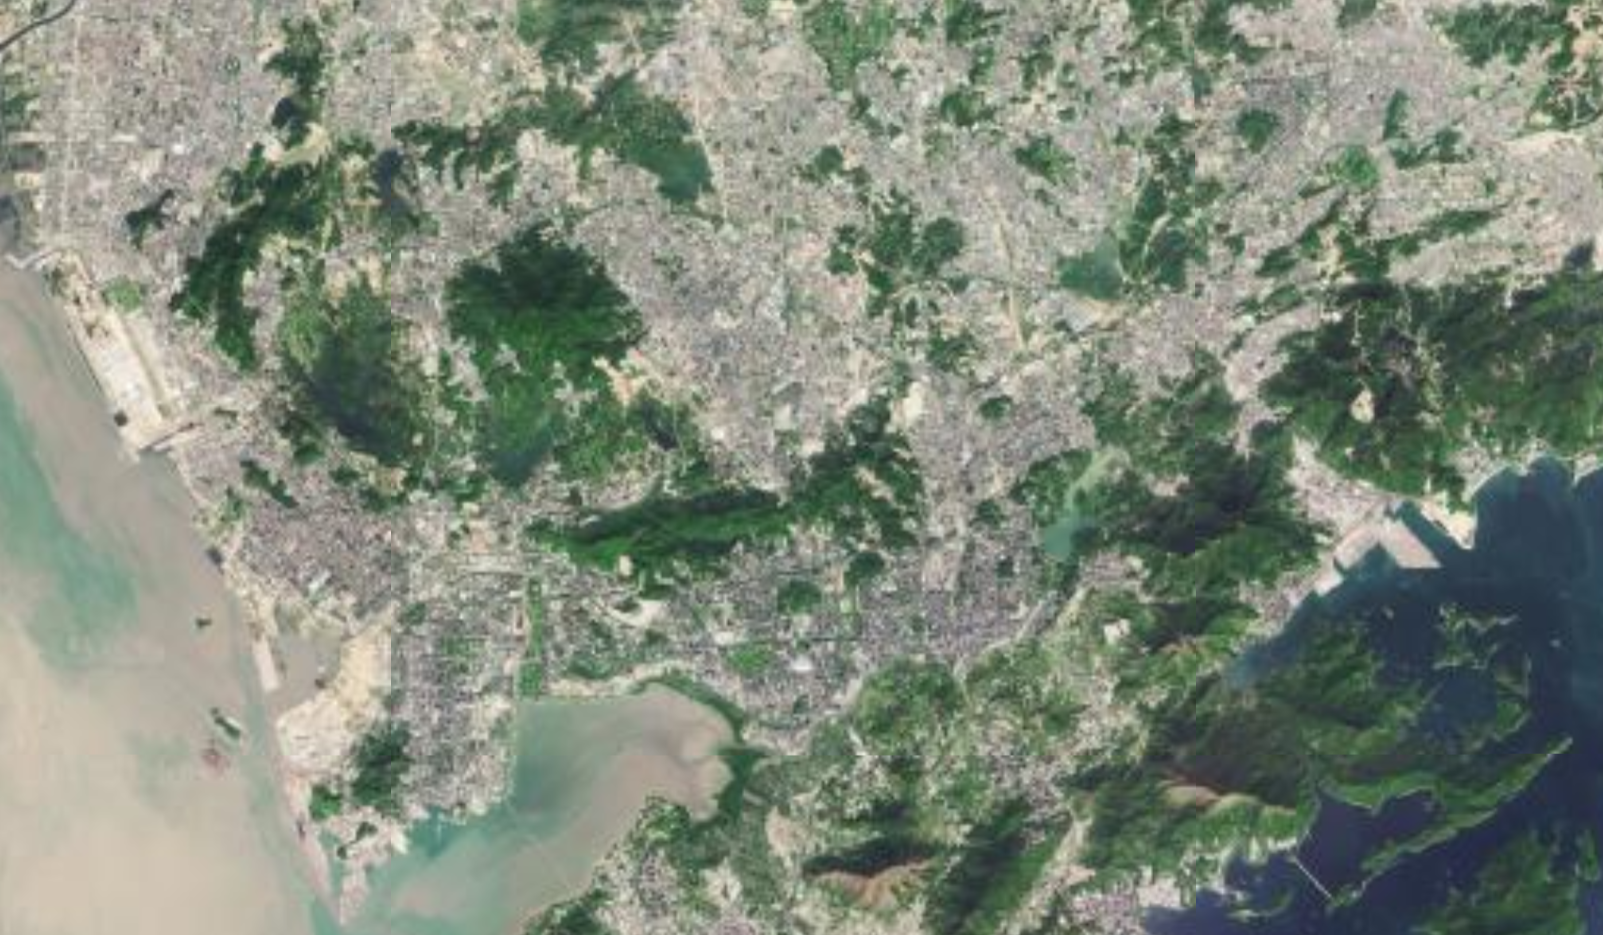
\includegraphics[width=0.85\textwidth]{chp02_影像地图.png}
  \caption{经过处理后的卫星遥感影像地图}
\end{figure}
  \end{onlyenv}

\vspace{-10pt}
  \begin{onlyenv}<2>
\begin{figure}
  \centering
  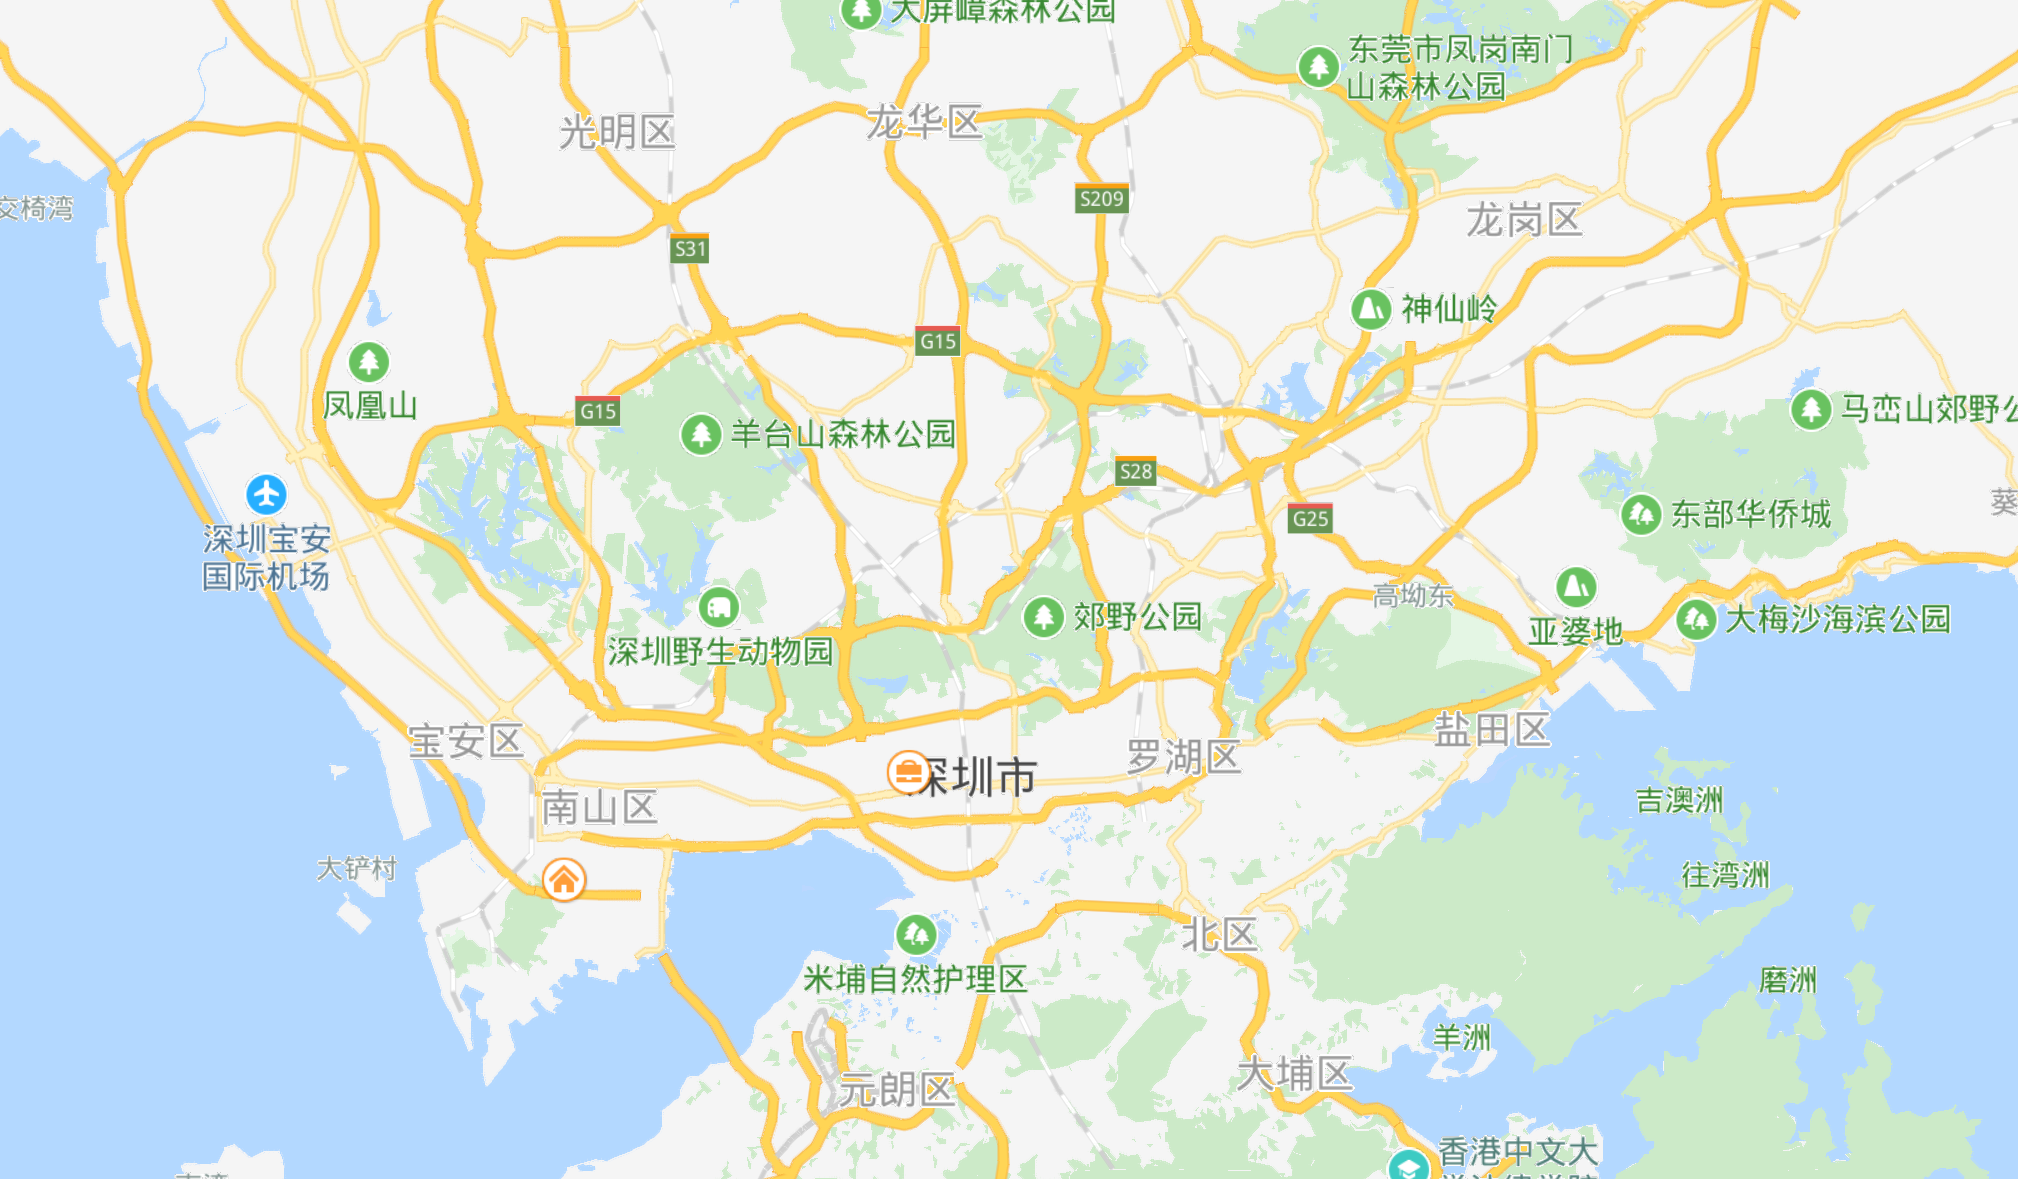
\includegraphics[width=0.85\textwidth]{chp02_瓦片地图.png}
  \caption{通过制图综合技术对矢量数据进行渲染优化,然后制作而成的瓦片地图}
\end{figure}
  \end{onlyenv}

  \begin{onlyenv}<3>
\begin{figure}
  \centering
  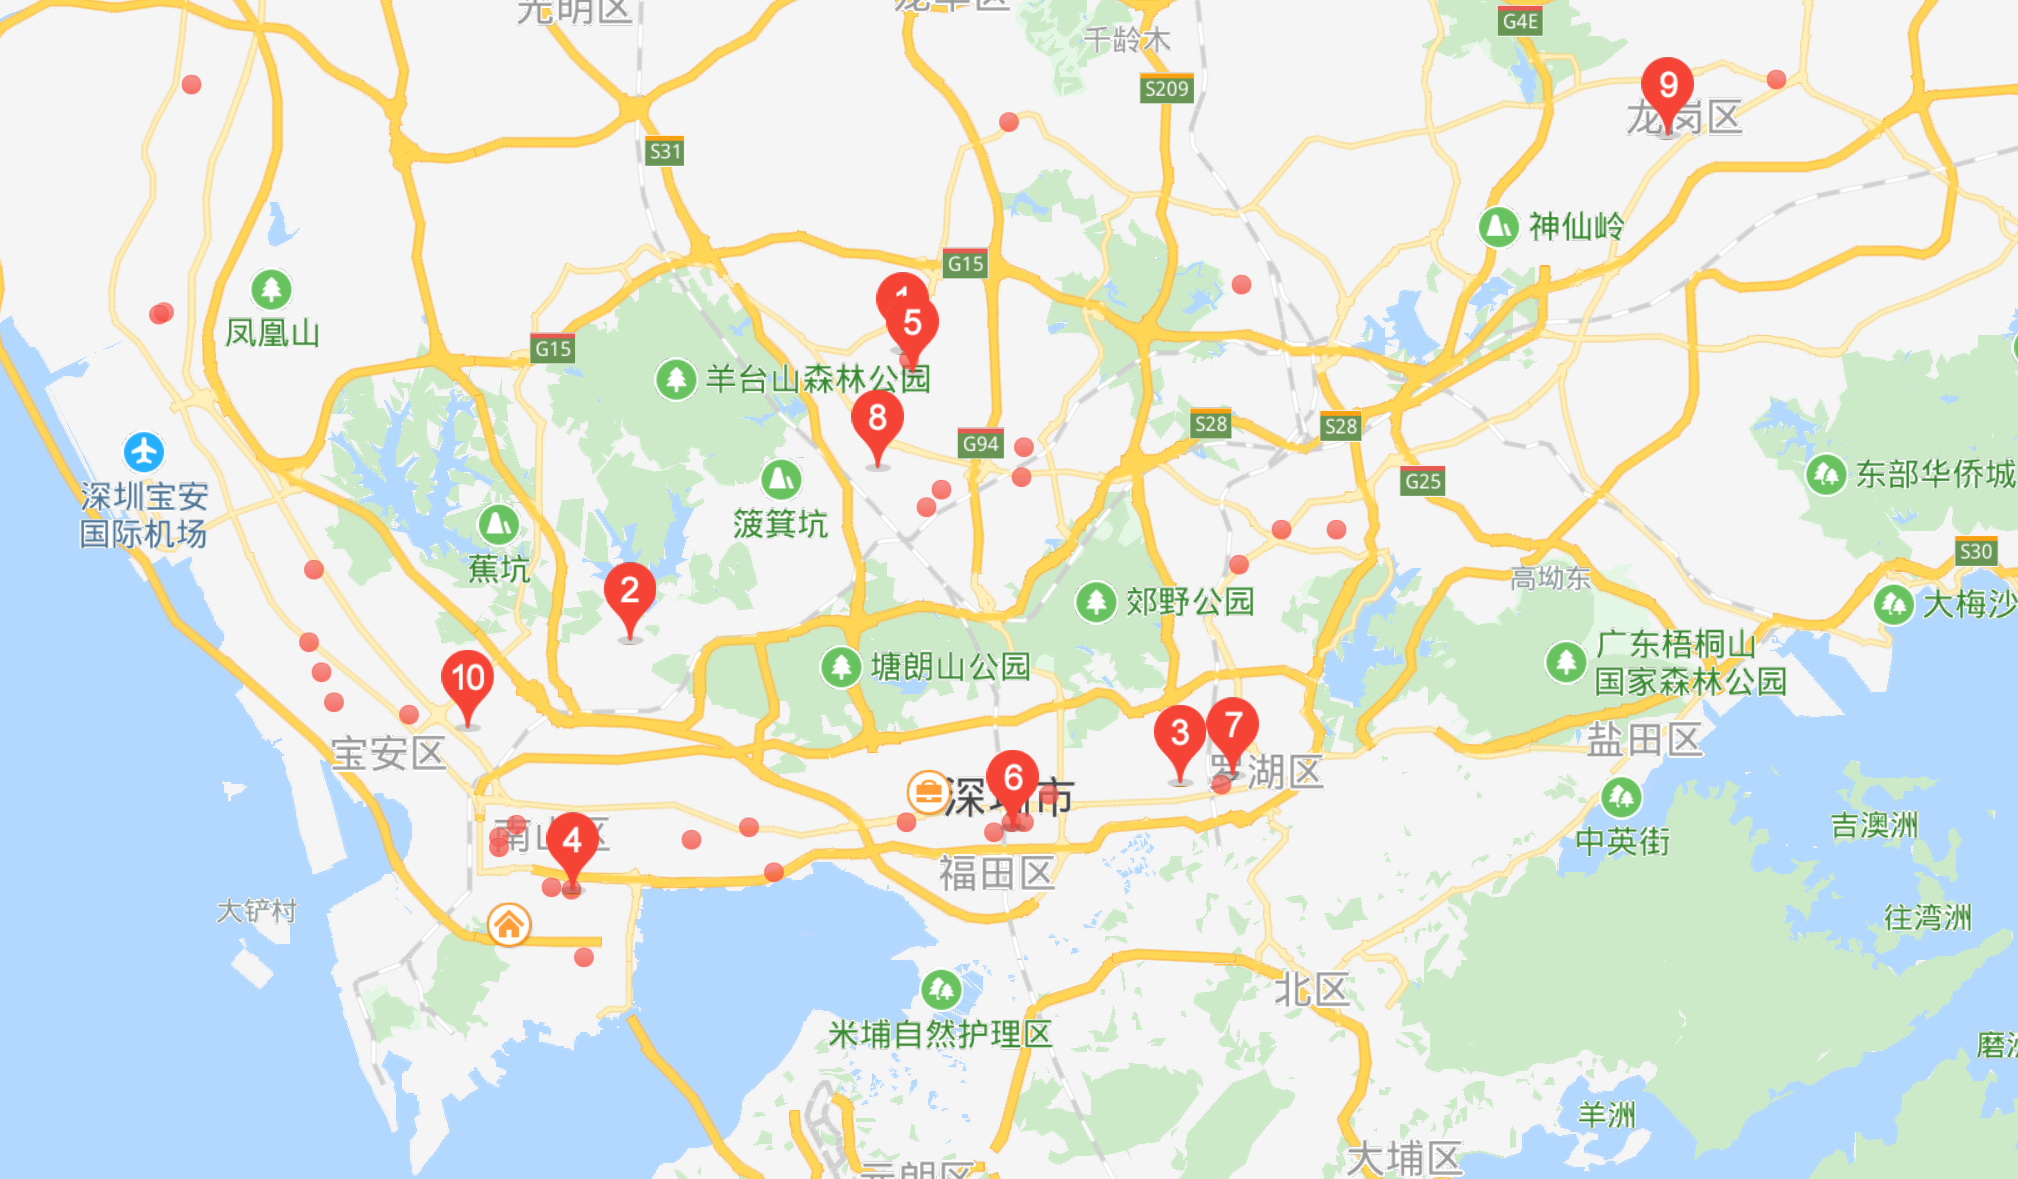
\includegraphics[width=0.85\textwidth]{chp02_兴趣点地图.png}
  \caption{兴趣点数据}
\end{figure}
  \end{onlyenv}

  \begin{onlyenv}<4>
\begin{figure}
  \centering
  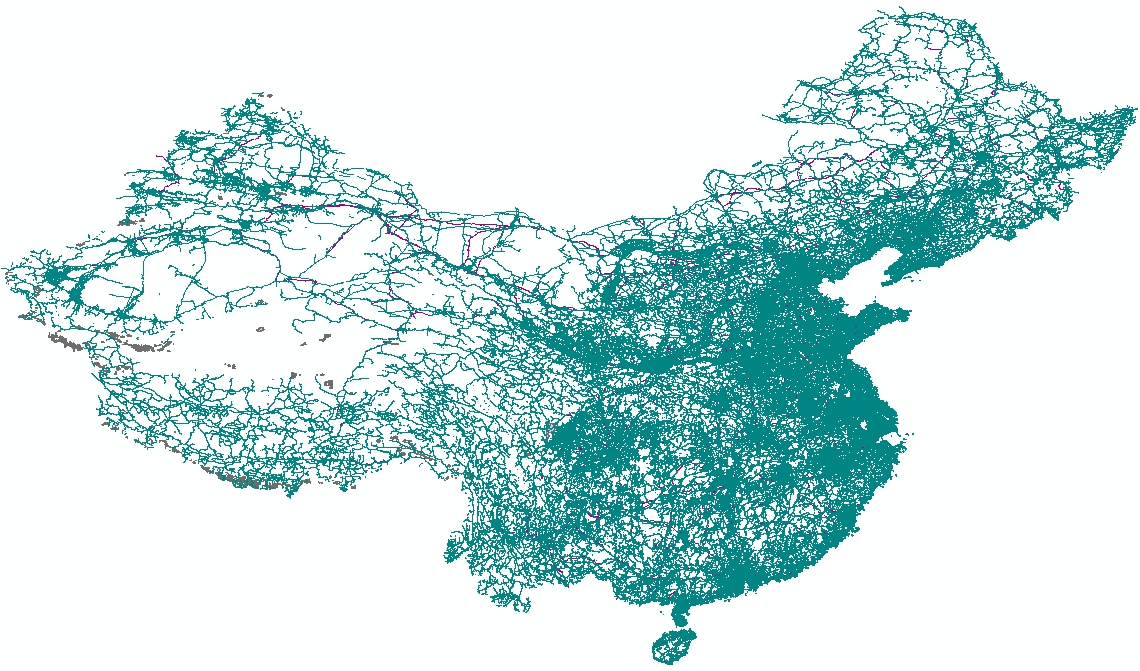
\includegraphics[width=0.8\textwidth]{chp02_OSM矢量地图.png}
  \caption{OSM网站获取的矢量GIS数据}
\end{figure}
  \end{onlyenv}
\end{overlayarea}

\end{frame}

\subsection{交通出行}


%
%%% Local Variables:
%%% mode: latex
%%% TeX-master: t
%%% End:
\section{数据分析的``武器库''}

\begin{frame}{\textcolor{white}{空白}}

  \begin{columns}
    \begin{column}{.5\textwidth}
      \begin{figure}
        \centering 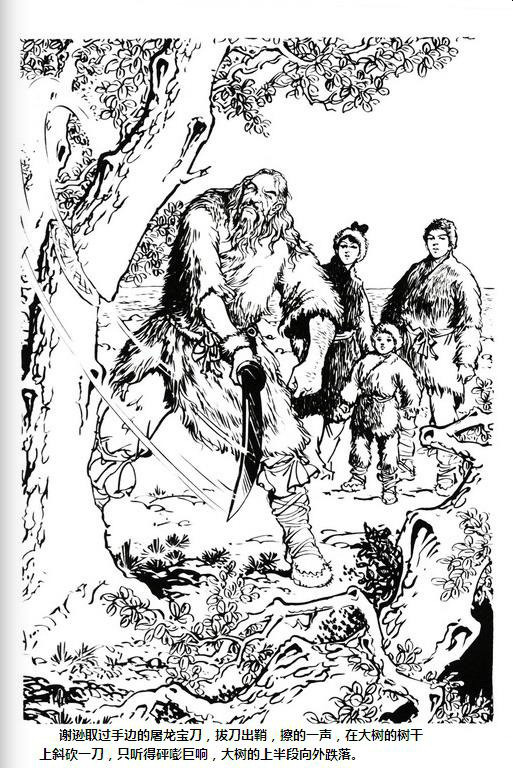
\includegraphics[width=0.95\columnwidth]{chp03_屠龙宝刀.jpg}
      \end{figure}
    \end{column}

    \begin{column}{.5\textwidth}
      \begin{ornamentblock}
        \centering
        {工欲善其事,必先利其器
          \rightline{\textemdash 《论语·卫灵公》}}
      \end{ornamentblock}
    \end{column}
  \end{columns}

\end{frame}

\begin{frame}{数据分析的``七种武器''}
\begin{enumerate}\large
\item 数据采集
\item 数据处理
\item 业务分析
\item 数据建模
\item 数据库
\item 分析算法
\item 可视化
\end{enumerate}
\end{frame}

\subsection{数据采集}
\begin{frame}[t]{\subsecname}
\begin{itemize}
\item<2-> 利用服务器端提供的API接口调取数据
\item<3-> 编写爬虫程序,从网页上抓取数据
\end{itemize}

\begin{overlayarea}{\textwidth}{\textheight}

  \begin{onlyenv}<2>
\begin{table} \centering \scriptsize
  \renewcommand\arraystretch{0.9}
  \begin{tabular}{|m{0.3\columnwidth}|m{0.3\columnwidth}|m{0.3\columnwidth}|}
    \toprule
    \rowcolor{LightCyan}
\multicolumn{1}{|c|}{\textbf{字段名称}} & \multicolumn{1}{c|}{\textbf{字段含义}} & \multicolumn{1}{c|}{\textbf{说明}}\\\hline
     alter & 交通出行方式 & 推荐公交、巴士优先、骑车、小汽车、出租车等 \\\hline
     O\_lon \& O\_lat & 出发地坐标 & 百度公司加密后的经纬度坐标 \\\hline
     D\_lon \& D\_lat & 到达地坐标 & 百度公司加密后的经纬度坐标 \\\hline
     distance & 出行距离 & 包括步行在内的实际路网距离\\\hline
     duration & 出行时间 & 包括步行在内 \\\hline
     price & 票价 & \\\hline
     walkDistance & 步行距离 & \\\hline
     walkTime & 步行时间 & \\\hline
     transferNumber & 换乘次数 & \\    
     \bottomrule
  \end{tabular}
\caption{百度地图API返回的公交路径规划数据结果}
\end{table}
  \end{onlyenv}

\vspace{-15pt}
  \begin{onlyenv}<3>
\begin{figure}
  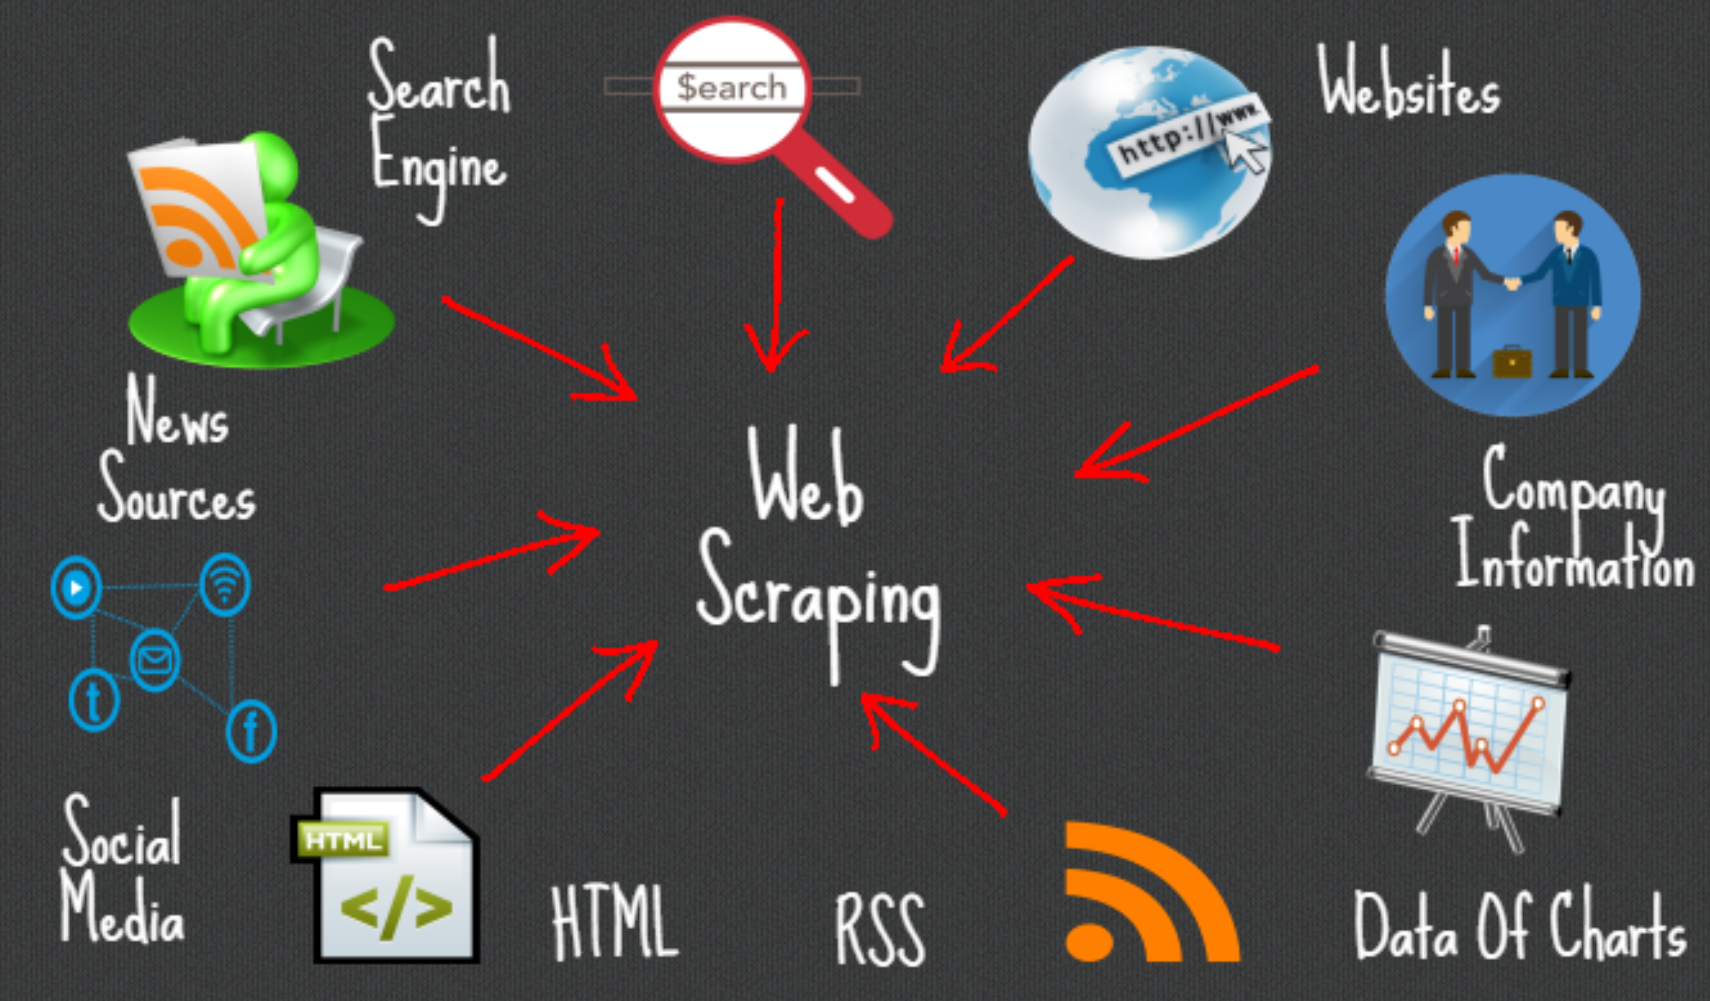
\includegraphics[width=\textwidth]{chp03_网络爬虫.png}
  \caption{利用爬虫程序,可以从丰富的互联网资源中自动化采集数据}
\end{figure}
  \end{onlyenv}
\end{overlayarea}

\end{frame}

\subsection{数据预处理}

\begin{frame}[t,fragile]{\subsecname}
\begin{itemize}
\item<1-> 现实中的原始数据都是不完整、不一致的脏数据,需要编写程序对数据进行\emphText{清洗、集成、变换和归约}等自动化处理
\item<2-> 示例:GPS数据预处理
\end{itemize}

\begin{overlayarea}{\textwidth}{\textheight}
  \begin{onlyenv}<2>
\begin{algorithm}[H] \tiny
     \SetKwInOut{Input}{输入}\SetKwInOut{Output}{输出}
     %\DontPrintSemicolon 
     \caption*{GPS原始数据清洗}
      
     \KwData{原始车牌GPS文件:GPS\_File,每行$line$=(ID,Postion,Time,Direction,Speed,State)}
     \KwResult{清洗后的GPS文件:GPS\_File\_P}
     \Input{时间容差$\Delta t$, 距离容差$\Delta d$,原始GPS数据列表$G$}
     \BlankLine

     \tcc{对$G$按照时间排序}
     SortByTime($G$)\;
     \BlankLine

     $bFirst$ $\leftarrow$ true\;

     \For{$i=1 \leftarrow 1$ \KwTo $N$}{
        \tcc{剔除位置不在市域范围$Rect$的错误点}
        \lIf{$G[i].position \notin Rect$}{\textbf{continue}}
           
        \eIf{$bFirst=true$}{
            GPS\_File\_P $\leftarrow$ OutputResult($G[i]$)\tcc*[r]{输出结果}
            $bFirst \leftarrow$ true; $tt \leftarrow G[i].time$; $tp \leftarrow G[i].position$;}
            {
            \tcc{根据前后点时间容差和距离容差剔除错误点}
            \If{$(5 \leqslant (G[i].time-tt) \leqslant{\Delta t}) \cap$
            Distance$(G[i].position,tp) \leqslant \Delta d$}
            {GPS\_File\_P $\leftarrow$ OutputResult($G[i]$)\tcc*[r]{输出结果} 
            $tt \leftarrow G[i].time$; $tp \leftarrow G[i].position$;}}
        }
\end{algorithm}
  \end{onlyenv}

  \begin{onlyenv}<3>
\begin{columns}
  \begin{column}{.4\textwidth}
\begin{figure}
  \centering
  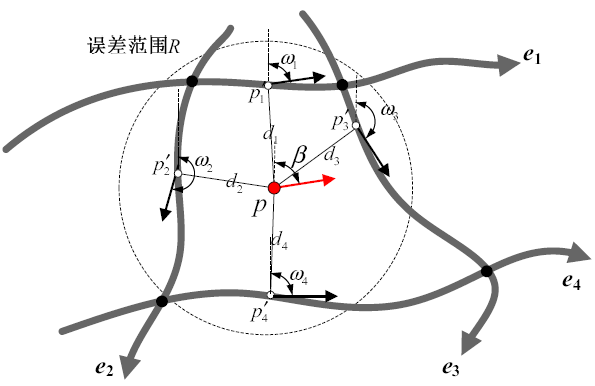
\includegraphics[width=\textwidth]{chp03_地图匹配示意.png}
\end{figure}
  \end{column}
  \begin{column}{.6\textwidth}
\begin{algorithm}[H] \tiny
     \SetKwInOut{Input}{输入}
     \SetKwInOut{Output}{输出}
     %\DontPrintSemicolon 
     \caption*{GPS与道路地图匹配}
     \Input{路网模型G和GPS轨迹$T$: $p_1 \rightarrow p_2 \rightarrow \cdots \rightarrow p_n$}
     \Output{处理后的GPS点序列$P$:$c_1^{j_1} \rightarrow c_2^{j_2} \rightarrow \cdots c_n^{j_n}$}
     \BlankLine    
     \tcc{清空列表$tList$}
     $tList \leftarrow empty$\; 
     \For{$i = 1$ \KwTo $n$}{
       \tcc{误差范围R内的候选路段集}
       $s$ = GetCandidates($p_i$,$G$,$R$)\; 
       $tList.add(s)$\;}
     $G_T^{\prime}$ = ConstructGraph($tList$)\tcc*[r]{构建图$G_T^{\prime}$}
     \Return FindMatchedSequence($G_T^{\prime}$)\;
\end{algorithm}
  \end{column}
\end{columns}
  \end{onlyenv}
\end{overlayarea}
\end{frame}

\subsection{业务分析}

\begin{frame}[t]{\subsecname}
\begin{itemize}
\item 数据分析中\emphText{最关键的环节}
\item 结合业务特点,确定待分析的内容和技术路线
\end{itemize}

\begin{figure}
  \centering
  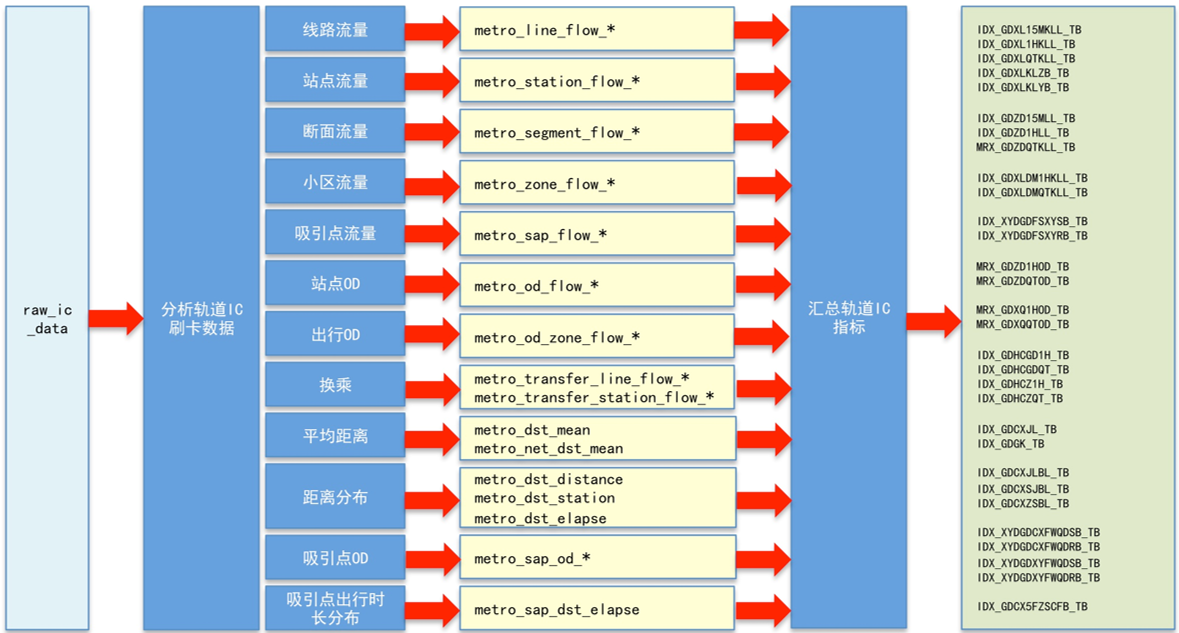
\includegraphics[width=\textwidth]{chp03_轨道刷卡业务分析.png}
  \caption{轨道刷卡数据分析的业务流程}
\end{figure}
\end{frame}

\subsection{数据建模}

\begin{frame}[t]{\subsecname}
\begin{itemize}
\item<1-> \emphText{根据业务需求对数据进行抽象},形成计算机能够理解的逻辑关系和物理结构
\item<2-> 示例:车辆轨迹模型 
\end{itemize}

\begin{overlayarea}{\textwidth}{\textheight}
  \begin{onlyenv}<2>
\begin{figure}
  \centering
  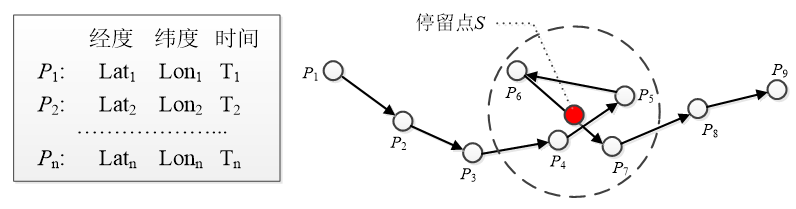
\includegraphics[width=0.8\textwidth]{chp03_停靠点提取算法.png} \\
  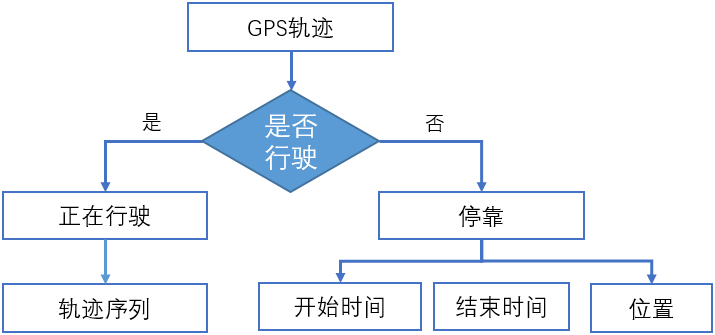
\includegraphics[width=0.6\textwidth]{chp03_GPS轨迹模型.png}
  \caption{车辆轨迹模型}
\end{figure}
  \end{onlyenv}
\end{overlayarea}
\end{frame}

\subsection{数据库}
\begin{frame}[t]{\subsecname}
\begin{itemize}
\item<1-> 通过高效的组织和存储,实现数据“增删改查”操作
\item<2-> 根据数据量级、数据内容、应用场景选择最适合的数据库技术
\item<3-> 数据库是大数据最核心的技术之一,目前主流采用\emphText{分布式存储方案}来解决
\end{itemize}

\begin{overlayarea}{\textwidth}{\textheight}
\vspace{-5pt}
  \begin{onlyenv}<1>
\begin{figure} \centering
\begin{columns}[b]
  \begin{column}{.5\textwidth}
    \begin{figure}
      
\includegraphics[height=0.4\textheight]{chp03_数据库技术1.png}
    \end{figure}
  \end{column}
  \begin{column}{.5\textwidth}
    \begin{figure}\flushleft
      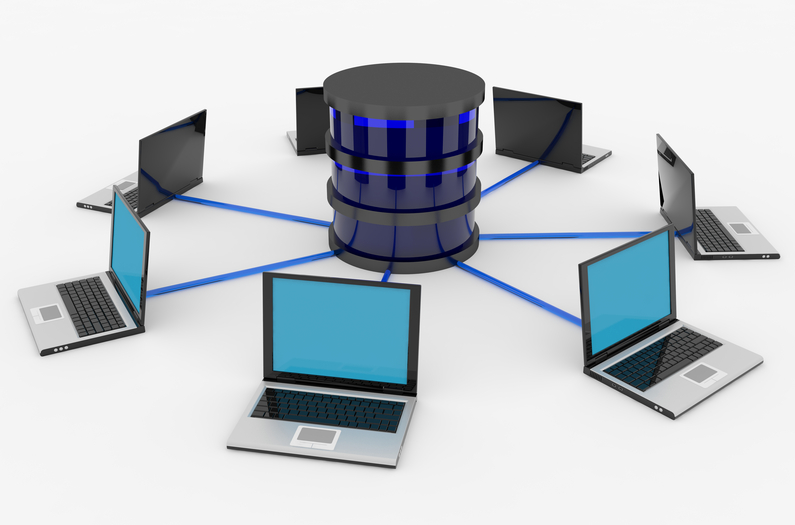
\includegraphics[height=0.35\textheight]{chp03_数据库技术2.png}
    \end{figure}
  \end{column}
\end{columns}
\caption{数据库技术的核心是对数据进行高效组织存储,以及多终端并发查询访问} 
\end{figure}
  \end{onlyenv}

\vspace{-10pt}
  \begin{onlyenv}<2>
\begin{figure}
  \centering
  
\includegraphics[width=0.7\textwidth]{chp03_数据库选择.png}
  \caption{根据实际需求选择最合适的数据库}
\end{figure}
  \end{onlyenv}

  \begin{onlyenv}<3>
\begin{figure}
  \centering
  
\includegraphics[width=0.8\textwidth]{chp03_大数据数据库产品.png}
  \caption{目前主流的大数据数据库产品}
\end{figure}
  \end{onlyenv}
\end{overlayarea}
\end{frame}

\subsection{分析算法}
\begin{frame}[t]{\subsecname}
\begin{itemize}
\item<1-> 算法不是简单的统计,而要能挖掘数据的规律和关系
\item<2-> 交通规划中最常用的分析算法是\emphText{空间分析算法}
\item<3-> 示例:核密度分析
\end{itemize}

  \begin{onlyenv}<3>
\begin{figure}
  \centering
  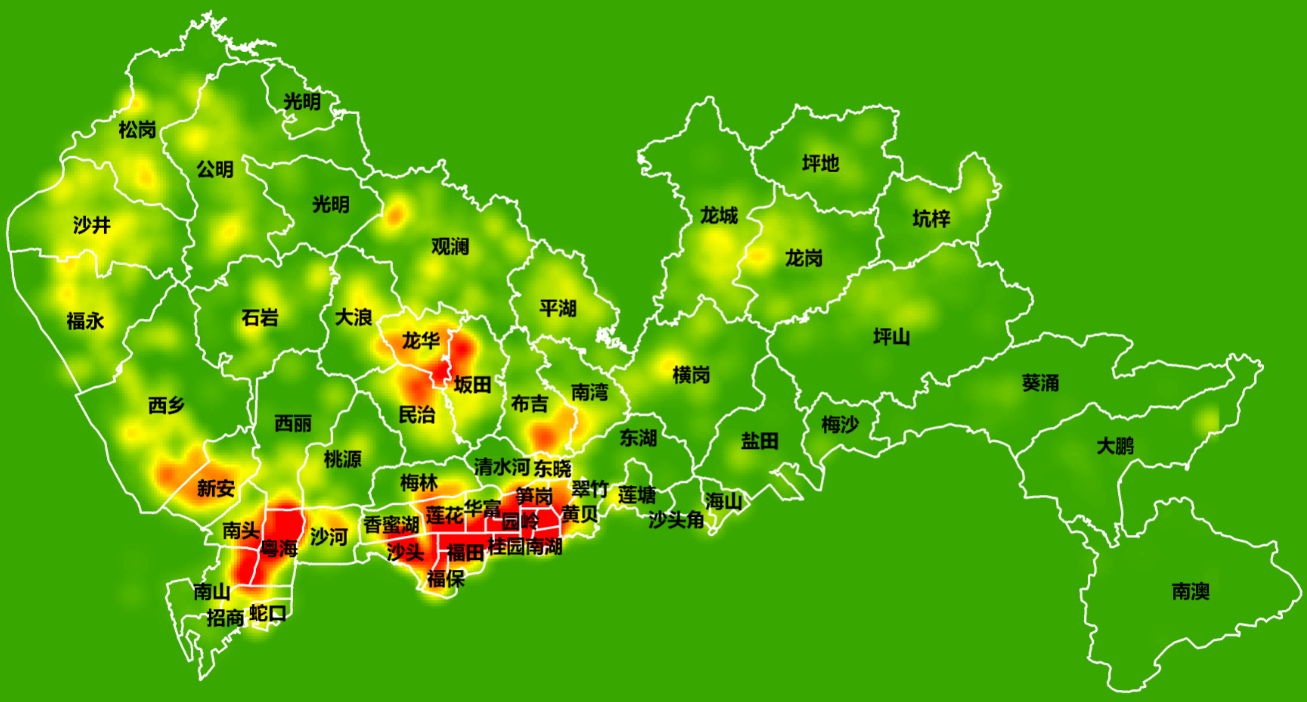
\includegraphics[width=0.9\textwidth]{chp03_核密度分析.png}
  \caption{核密度分析}
\end{figure}
  \end{onlyenv}

\only<4>{
    \begin{columns}[c]
      \begin{column}{0.4\textwidth}
         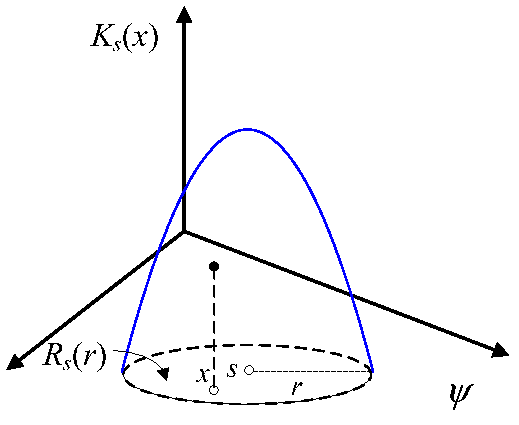
\includegraphics[width=1\columnwidth]{chp03_KDE模型.pdf}
      \end{column}

      \begin{column}{0.6\textwidth}
         \begin{beamerboxesrounded}{\small 带权重的核密度估计 \footnotemark[1]$^,$\footnotemark[2]}\scriptsize
           \[\hat \lambda (s) = \frac{1}{{n\pi {r^2}}}\sum\nolimits_{i = 1}^n {{w_i}{K_s}\left( {\frac{{{d_{sx}}}}{r}} \right)}\]
           其中,${d_{sx}} = \left\| {s - {x_i}} \right\|$表示位置$s$和第$i$个样本$x_i$之间的欧式距离;$r$被称为带宽,表示区域${R_s}(r)$的面积大小。
         \end{beamerboxesrounded}
      \end{column}
    \end{columns}

    \begin{itemize} \tiny
      \item KDE的核心思想就是通过计算单位面积内样本的核密度平滑处理来估计位置的属性值
      \item KDE结果表示区域${R_s}(r)$内不同样本对估计$s$ 位置属性值的权重
      \item 核函数是一个与距离有关的函数,而且其赋予区域${R_s}(r)$内每个样本点的值是不同的,离中心位置$s$ 越远的样本点,其值应该越小,而离中心位置$s$越近的样本点,其值应该越大
      \item 对KDE结果产生影响的两个因素包括核函数的形式以及带宽的选择
    \end{itemize}

\vspace{5pt}
    \footnotetext[1]{\tiny Silverman B W. 1986. Density Estimation for Statistics and Data Analysis[M]. London: Chapman Hall.}
    \footnotetext[2]{\tiny Wand M P, Jones M C. 1995. Kernel Smoothing[M]. Boca Raton, Florida: Chapman \& Hall/CRC. }}

\only<5>{
   \begin{figure}
       \subfloat[Uniform]
           {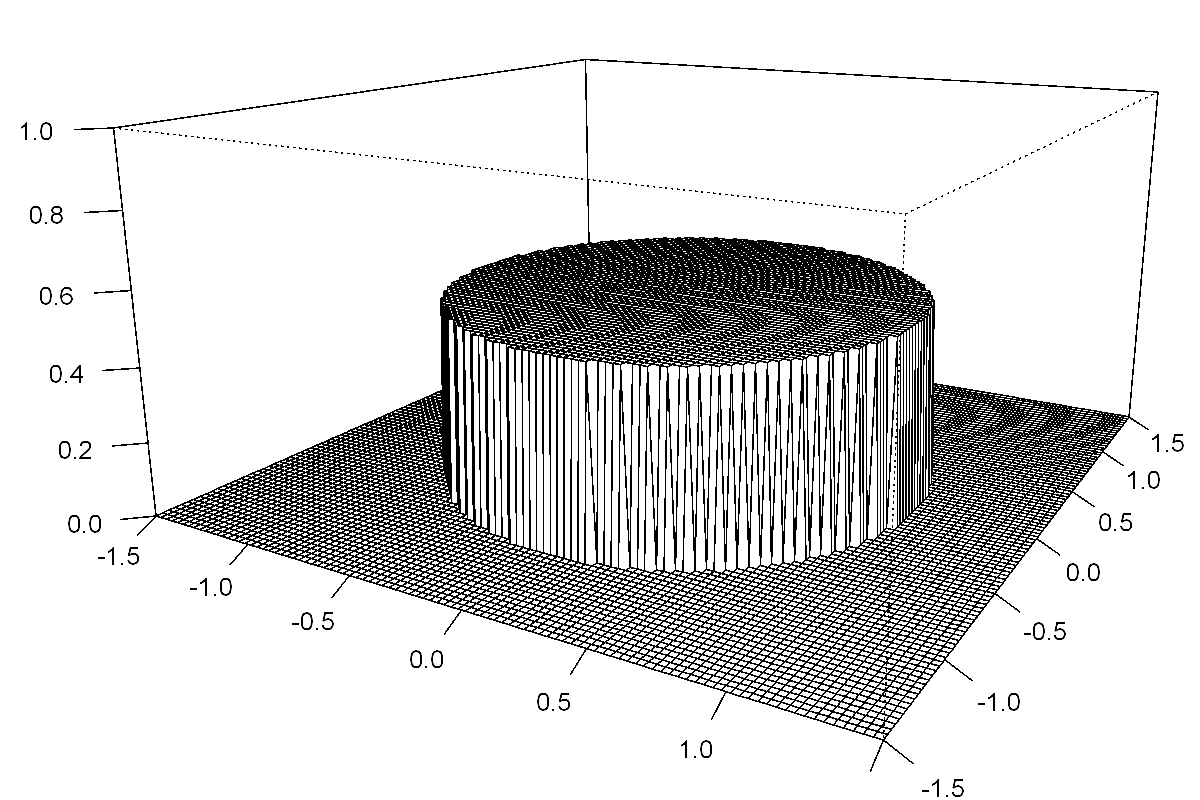
\includegraphics[width=0.24\columnwidth]
           {chp03_Function_Uniform.pdf}}\vspace{0.5pt}
       \subfloat[Triangular]
           {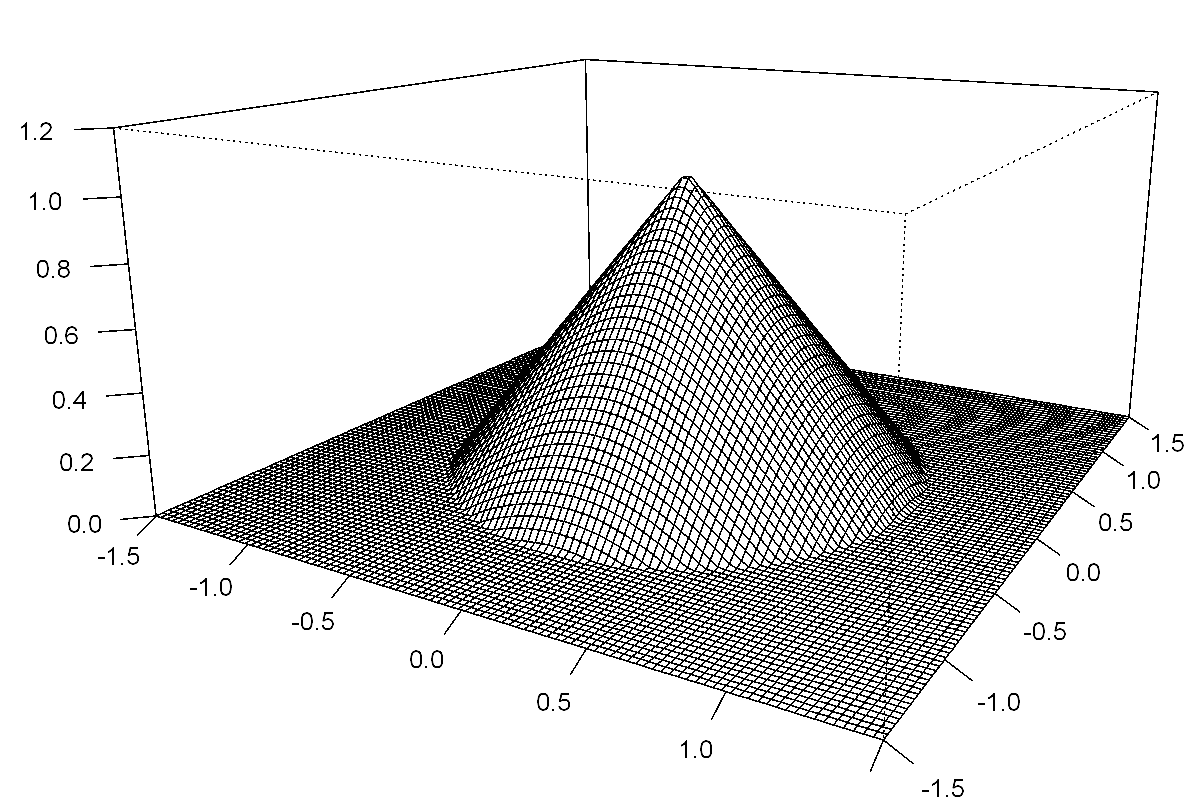
\includegraphics[width=0.24\columnwidth]
           {chp03_Function_Triangular.pdf}}\vspace{0.5pt}
       \subfloat[Quartic]
           {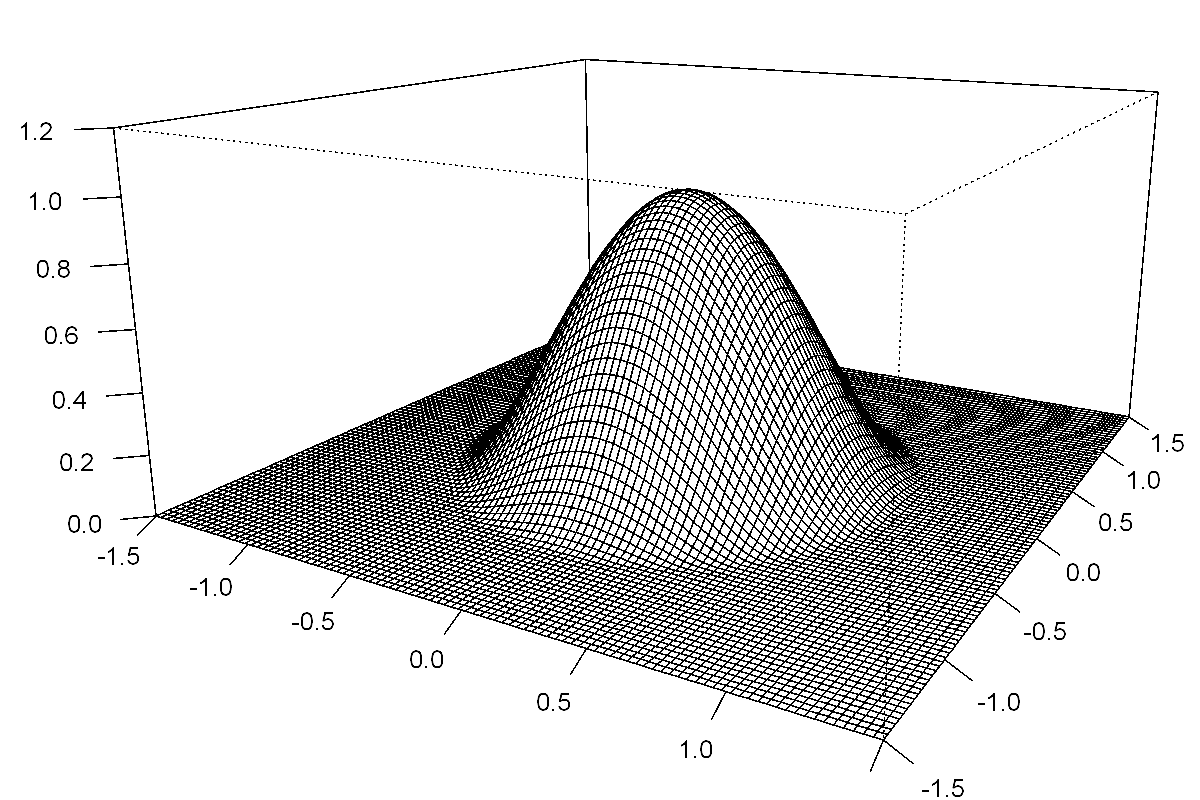
\includegraphics[width=0.24\columnwidth]
           {chp03_Function_Quartic.pdf}} \vspace{0.5pt}
       \subfloat[Triweight]
           {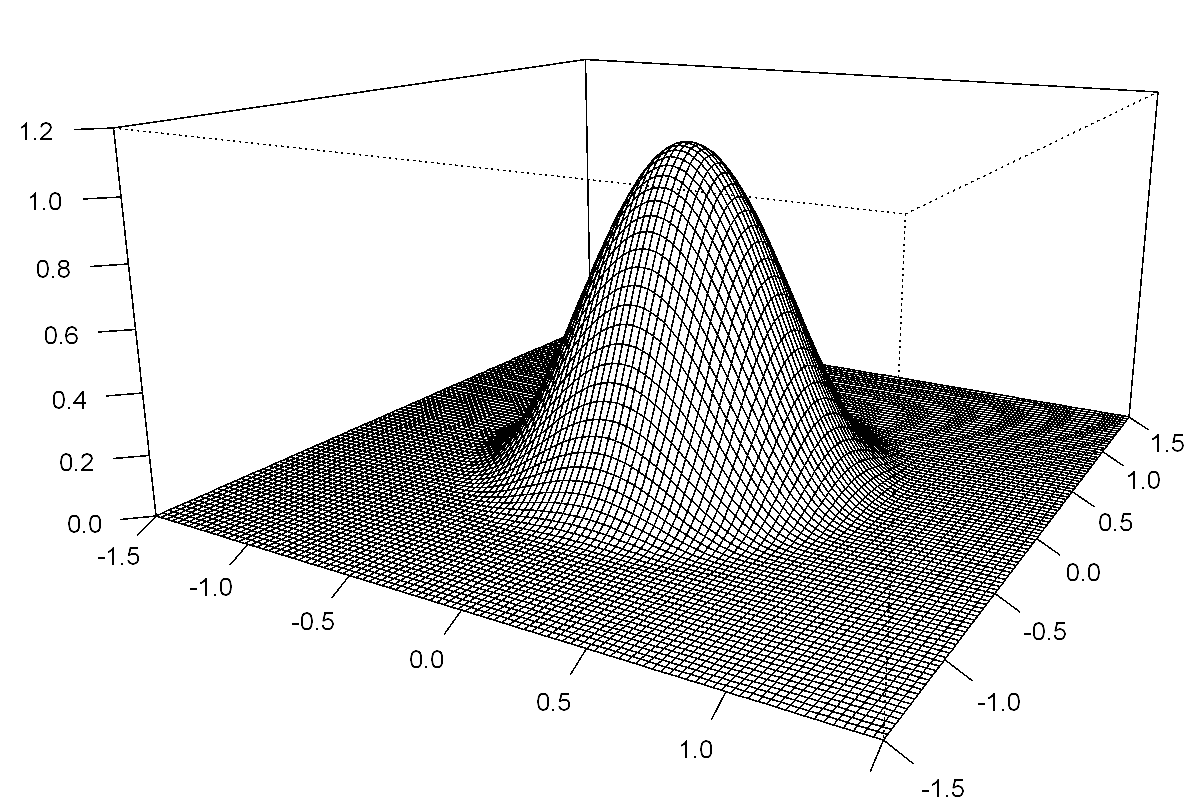
\includegraphics[width=0.24\columnwidth]
           {chp03_Function_Triweight.pdf}} \\
       \subfloat[Tricube]
           {\includegraphics[width=0.24\columnwidth]
           {chp03_Function_Tricube.pdf}}  \vspace{0.5pt}
       \subfloat[Epanechnikov]
           {\includegraphics[width=0.24\columnwidth]
           {chp03_Function_Epanechnikov.pdf}} \vspace{0.5pt}
       \subfloat[Gaussian]
           {\includegraphics[width=0.24\columnwidth]
           {chp03_Function_Gaussian.pdf}}   \vspace{0.5pt}
       \caption{常见的核函数}
   \end{figure}}
\end{frame}

\subsection{可视化}
\begin{frame}[t]{\subsecname}
\begin{itemize}
\item<1-> 计算机技术与艺术的结合
\item<2-> \emphText{将绘图与数据分离,数据相关绘图与数据无关绘图分离}
\item<3-> 示例:变形地图(cartogram)
\end{itemize}

\begin{overlayarea}{\textwidth}{\textheight}
  \begin{onlyenv}<1>
  \begin{columns}
    \begin{column}{.4\textwidth}
      \begin{figure}
        \centering \includegraphics[width=\columnwidth]{chp03_edward_tufte.png}
        \caption{\scriptsize Edward Tufte(1942-),美国统计学家,数据可视化理论的先驱者和领军人物,人称“数据
    达芬奇”}
      \end{figure}
    \end{column}

    \begin{column}{.6\textwidth}
  \begin{ornamentblock}
    {The commonality between science and art is in trying to see profoundly - to develop strategies of seeing and showing.\\
      \rightline{\textemdash Edward Tufte}}
  \end{ornamentblock}
    \end{column}
  \end{columns}
  \end{onlyenv}

\vspace{-10pt}
  \begin{onlyenv}<2>
\begin{figure}[ht]
  \centering
  \includegraphics[width=0.7\columnwidth]{chp03_the_grammar_of_graphics.png}
  \caption{可视化领域经典著作《The Grammar of Graphics》的第一版(1999)和第二版(2005)}
\end{figure}
  \end{onlyenv}

\vspace{-10pt}
  \begin{onlyenv}<3>
\begin{figure}
  \centering
  \includegraphics[width=0.8\textwidth]{chp04_人口.png}
  \caption{深莞街道人口密度}
\end{figure}
  \end{onlyenv}

  \begin{onlyenv}<4>
\begin{figure}
  \centering
  \includegraphics[width=0.7\textwidth]{chp04_人口密度cartogram.jpg}
  \caption{深莞街道人口密度变形地图(cartogram)}
\end{figure}
  \end{onlyenv}

  \begin{onlyenv}<5>
\begin{figure}
  \centering
  \includegraphics[width=0.8\textwidth]{chp04_岗位.png}
  \caption{深莞街道岗位密度}
\end{figure}
  \end{onlyenv}

  \begin{onlyenv}<6>
\begin{figure}
  \centering
  \includegraphics[width=0.7\textwidth]{chp04_岗位密度cartogram.jpg}
  \caption{深莞街道岗位密度变形地图(cartogram)}
\end{figure}
  \end{onlyenv}
%   \begin{onlyenv}<3>
% \begin{figure}[ht]
%   \centering
%   \includegraphics[width=\columnwidth]{chp03_流量可视化.png}
%   \caption{在一张图中同时展现总流量、OD量和内外部出行比例,数据在外部单独存储,与样式无关}
% \end{figure}
%   \end{onlyenv}
\end{overlayarea}
\end{frame}



%%% Local Variables:
%%% mode: latex
%%% TeX-master: t
%%% End:
\section{数据在业务中的应用案例}

\subsection{常规交通指标分析}

\begin{frame}[t]{\subsecname}
  \begin{itemize}
     \item<1->出租车
        \begin{enumerate}
          \item 客流量分析(乘次、产生量和吸引量统计)
          \item 出行分析(OD矩阵、OD行程时间和出行距离)
          \item 运营分析(空驶比例、路段行程车速)
        \end{enumerate}
     \item<2->定点车流
        \begin{enumerate}
          \item 流量统计
          \item 流量时变分析
          \item 流向分析(各关口每日出入关的总流量)
        \end{enumerate}
     \item<3->常规公交
        \begin{enumerate}
          \item 客流量分析(线路、站点、换乘)
          \item 出行分析(站点OD、出行OD)
          \item 运营分析(车速、发车频率、候车时间)
          \item 可达性分析
          \item 站点覆盖范围分析
        \end{enumerate}
     \item<4->轨道
        \begin{enumerate}
          \item 客流量统计
          \item 出行统计(站点OD、出行OD、OD行程时间、出行距离)
          \item 运营统计(线路拥挤度、站点拥挤度)
        \end{enumerate}
  \end{itemize}
\end{frame}

\begin{frame}[t]{\subsecname}
  \begin{itemize}
     \item<1-> 居民出行调查
        \begin{enumerate}
          \item 人口、就业、年龄、收入等分布
          \item 交通方式和交通目的比例
          \item 分交通方式和交通目的的出行量
          \item 通勤交通分析 
        \end{enumerate}
  \end{itemize}
  \begin{itemize}
     \item<2-> 手机
        \begin{enumerate}
          \item 就业和居住人口分布
          \item 不分交通方式和目的的出行量
          \item 通勤交通分析 
        \end{enumerate}
  \end{itemize}

\only<3>{
\begin{badbox}{多种数据融合使用} 
   当遇到同一指标存在多种数据源都可以计算的情况,针对应用场景选择最合适的数据进行计算
\end{badbox}}
\end{frame}

\subsection{都市圈范围分析}

\begin{frame}[t]{\subsecname}
\begin{itemize}
  \item<1-> 数据:2010和2016年居民出行调查
  \item<2-> 分析指标:通勤率=某区域至中心区域通勤人数/该区域常住人口
  \item<3-> 解决问题:深圳市城市边界的空间增长与发展规律
\end{itemize}

\end{frame}

\subsection{区域联系强度分析}

\subsection{货运交通分析}




%%%%%%%%%%%%%%%%%%%%%%%%%%%%%%%%%%%%%%%%%%%%%%%%%%%%%%%%%%%%

%%%%%%%%%%%%%%%%%%%%%%%%%%%%%%%%%%%%%%%%%%%%%%%%%%%%%%%%%%%%


%%%%%%%%%%%%%%%%%%%%%%%%%%%%%%%%%%%%%%%%%%%%%%%%%%%%%%%%%%%%

%%%%%%%%%%%%%%%%%%%%%%%%%%%%%%%%%%%%%%%%%%%%%%%%%%%%%%%%%%%%


%%%%%%%%%%%%%%%%%%%%%%%%%%%%%%%%%%%%%%%%%%%%%%%%%%%%%%%%%%%%

%%%%%%%%%%%%%%%%%%%%%%%%%%%%%%%%%%%%%%%%%%%%%%%%%%%%%%%%%%%%
\section{再认识与展望}

%%%%%%%%%%%%%%%%%%%%%%%%%%%%%%%%%%%%%%%%%%%%%%%%%%%%%%%%%%%%

%%%%%%%%%%%%%%%%%%%%%%%%%%%%%%%%%%%%%%%%%%%%%%%%%%%%%%%%%%%%

%%%%%%%%%%%%%%%%%%%%%%%%%%%%%%%%%%%%%%%%%%%%%%%%%%%%%%%%%%%%%%%%%%%%%%%%%%%%
% 结束页
%%%%%%%%%%%%%%%%%%%%%%%%%%%%%%%%%%%%%%%%%%%%%%%%%%%%%%%%%%%%%%%%%%%%%%%%%%%%
\begin{frame}[plain,noframenumbering]%
  \finalpage{
    \begin{table} \Huge \centering
      \begin{tabular}{c}
        汇~报~结~束\\
        谢~谢!
      \end{tabular} \end{table}
    \titlegraphic{\pgfuseimage{mainlogo}}}
\end{frame}
\end{document}
%%% Local Variables:
%%% mode: latex
%%% TeX-master: t
%%% End:
